        %%******************************************%%
        %%                                          %%
        %%        Modello di tesi di laurea         %%
        %%            di Andrea Giraldin            %%
        %%                                          %%
        %%             2 novembre 2012              %%
        %%                                          %%
        %%******************************************%%


% I seguenti commenti speciali impostano:
% 1. 
% 2. PDFLaTeX come motore di composizione;
% 3. tesi.tex come documento principale;
% 4. il controllo ortografico italiano per l'editor.

% !TEX encoding = UTF-8
% !TEX TS-program = pdflatex
% !TEX root = tesi.tex
% !TEX spellcheck = it-IT

\documentclass[11pt,                    % corpo del font principale
               a4paper,                 % carta A4
               twoside,                 % impagina per fronte-retro
               openright,               % inizio capitoli a destra
               english,                 
               italian,                 
               ]{book}    

\usepackage[utf8]{inputenc}             % codifica di input; anche [latin1] va bene
                                        % NOTA BENE! va accordata con le preferenze dell'editor

%**************************************************************
% Importazione package
%************************************************************** 

%\usepackage{amsmath,amssymb,amsthm}    % matematica

\usepackage[english, italian]{babel}    % per scrivere in italiano e in inglese;
                                        % l'ultima lingua (l'italiano) risulta predefinita

\usepackage{bookmark}                   % segnalibri

\usepackage{caption}                    % didascalie

\usepackage{chngpage,calc}              % centra il frontespizio

\usepackage{csquotes}                   % gestisce automaticamente i caratteri (")

\usepackage{emptypage}                  % pagine vuote senza testatina e piede di pagina

\usepackage{epigraph}					% per epigrafi

\usepackage{eurosym}                    % simbolo dell'euro

\usepackage[T1]{fontenc}                % codifica dei font:
                                        % NOTA BENE! richiede una distribuzione *completa* di LaTeX

\usepackage{graphicx}                   % immagini

\usepackage{hyperref}                   % collegamenti ipertestuali



\usepackage[binding=5mm]{layaureo}      % margini ottimizzati per l'A4; rilegatura di 5 mm

\usepackage{listings}                   % codici

\usepackage{microtype}                  % microtipografia

\usepackage{mparhack,relsize}  % finezze tipografiche

\usepackage{nameref}                    % visualizza nome dei riferimenti                                      

\usepackage[font=small]{quoting}        % citazioni

\usepackage{subfig}                     % sottofigure, sottotabelle

\usepackage[italian]{varioref}          % riferimenti completi della pagina

\usepackage[dvipsnames]{xcolor}         % colori

\usepackage{booktabs}                   % tabelle                                       
\usepackage{tabularx}                   % tabelle di larghezza prefissata                                    
\usepackage{longtable}                  % tabelle su più pagine                                        
\usepackage{ltxtable}                   % tabelle su più pagine e adattabili in larghezza

\usepackage[toc, acronym]{glossaries}   % glossario
                                        % per includerlo nel documento bisogna:
                                        % 1. compilare una prima volta tesi.tex;
                                        % 2. eseguire: makeindex -s tesi.ist -t tesi.glg -o tesi.gls tesi.glo
                                        % 3. eseguire: makeindex -s tesi.ist -t tesi.alg -o tesi.acr tesi.acn
                                        % 4. compilare due volte tesi.tex.

\usepackage[backend=biber,style=verbose-ibid,hyperref,backref]{biblatex}
                                        % eccellente pacchetto per la bibliografia; 
                                        % produce uno stile di citazione autore-anno; 
                                        % lo stile "numeric-comp" produce riferimenti numerici
                                        % per includerlo nel documento bisogna:
                                        % 1. compilare una prima volta tesi.tex;
                                        % 2. eseguire: biber tesi
                                        % 3. compilare ancora tesi.tex.

%**************************************************************
% file contenente le impostazioni della tesi
%**************************************************************

%**************************************************************
% Frontespizio
%**************************************************************
\newcommand{\myName}{Andrea Tombolato}                          % autore
\newcommand{\myID}{1069144}																			% matricola
\newcommand{\myTitle}{Refactoring di una piattaforma CMS: database MySQL, API REST ed interfaccia grafica}                    
\newcommand{\myDegree}{Tesi di laurea triennale}                % tipo di tesi
\newcommand{\myUni}{Università degli Studi di Padova}           % università
\newcommand{\myFaculty}{Corso di Laurea in Informatica}         % facoltà
\newcommand{\myDepartment}{Dipartimento di Matematica}          % dipartimento
\newcommand{\myProf}{Ombretta Gaggi}                            % relatore
\newcommand{\myLocation}{Padova}                                % dove
\newcommand{\myAA}{2015-2016}                                   % anno accademico
\newcommand{\myTime}{Agosto 2016}                               % quando

\usepackage{lipsum}

\newcommand\textbox[1]{%
  \parbox{.333\textwidth}{#1}%
}


%**************************************************************
% Impostazioni di impaginazione
% see: http://wwwcdf.pd.infn.it/AppuntiLinux/a2547.htm
%**************************************************************

\setlength{\parindent}{14pt}   % larghezza rientro della prima riga
\setlength{\parskip}{0pt}   % distanza tra i paragrafi


%**************************************************************
% Impostazioni di biblatex
%**************************************************************
\bibliography{bibliografia} % database di biblatex 

\defbibheading{bibliography}
{
    \cleardoublepage
    \phantomsection 
    \addcontentsline{toc}{chapter}{\bibname}
    \chapter*{\bibname\markboth{\bibname}{\bibname}}
}

\setlength\bibitemsep{1.5\itemsep} % spazio tra entry

\DeclareBibliographyCategory{opere}
\DeclareBibliographyCategory{web}

\addtocategory{opere}{atzeni:basi-di-dati}
\addtocategory{opere}{gang:design-patterns}
\addtocategory{web}{site:laravel-doc}

\defbibheading{opere}{\section*{Riferimenti bibliografici}}
\defbibheading{web}{\section*{Siti Web consultati}}


%**************************************************************
% Impostazioni di caption
%**************************************************************
\captionsetup{
    tableposition=top,
    figureposition=bottom,
    font=small,
    format=hang,
    labelfont=bf
}

%**************************************************************
% Impostazioni di glossaries
%**************************************************************

%**************************************************************
% Acronimi
%**************************************************************
\renewcommand{\acronymname}{Acronimi e abbreviazioni}

\newacronym[description={\glslink{apig}{Application Programming Interface}}]
    {api}{API}{Application Programming Interface}

\newacronym[description={\glslink{umlg}{Unified Modeling Language}}]
    {uml}{UML}{Unified Modeling Language}
		
\newacronym[description={\glslink{b2bg}{Business-to-Business}}]
    {b2b}{B2B}{Business-to-Business}
		
\newacronym[description={\glslink{iotg}{Intenet of Things}}]
    {iot}{IoT}{Intenet of Things}

%**************************************************************
% Glossario
%**************************************************************
%\renewcommand{\glossaryname}{Glossario}

\newglossaryentry{apig}
{
    name=\glslink{api}{API},
    text=Application Programming Interface,
    sort=api,
    description={in informatica con il termine \emph{Application Programming Interface API} (ing. interfaccia di programmazione di un'applicazione) si indica ogni insieme di procedure disponibili al programmatore, di solito raggruppate a formare un set di strumenti specifici per l'espletamento di un determinato compito all'interno di un certo programma. La finalità è ottenere un'astrazione, di solito tra l'hardware e il programmatore o tra software a basso e quello ad alto livello semplificando così il lavoro di programmazione}
}

\newglossaryentry{umlg}
{
    name=\glslink{uml}{UML},
    text=UML,
    sort=uml,
    description={in ingegneria del software \emph{UML, Unified Modeling Language} (ing. linguaggio di modellazione unificato) è un linguaggio di modellazione e specifica basato sul paradigma object-oriented. L'\emph{UML} svolge un'importantissima funzione di ``lingua franca'' nella comunità della progettazione e programmazione a oggetti. Gran parte della letteratura di settore usa tale linguaggio per descrivere soluzioni analitiche e progettuali in modo sintetico e comprensibile a un vasto pubblico}
}

\newglossaryentry{startupg}
{
    name=Startup,
    text=startup,
    sort=startup,
    description={in economia, con questo termine, si indica una nuova impresa nelle forme di un'organizzazione temporanea o una società di capitali in cerca di un business model ripetibile e scalabile.
La scalabilità è un elemento cardine di questa tipologia di impresa. L'avvio di un'attività imprenditoriale non scalabile, come l'apertura di un ristorante, non coincide dunque con la creazione di una startup ma, piuttosto, di una società tradizionale}
}

\newglossaryentry{b2bg}
{
    name=B2B,
    text=B2B,
    sort=Business-to-Business,
    description={ acronimo di “\emph{business-to-business}”. Locuzione utilizzata per descrivere le transazioni commerciali elettroniche tra imprese, distinguendole da quelle che intercorrono tra le imprese e altri gruppi, come quelle tra una ditta e i clienti individuali (B2C, acronimo di “\emph{business-to-consumer}”) oppure quelle tra una impresa e il governo (B2G, acronimo di “\emph{business-to-government}”)}
}

\newglossaryentry{earlystageg}
{
    name=Finanziamento early stage,
    text=finanziamento early stage,
    sort=finanziamento,
    description={ investimento atto a sostenere le fasi iniziali di un’azienda o di un business}
}

\newglossaryentry{iotg}
{
    name=IoT, %voce glossario
    text=IoT, %sostituisce parola nel testo
    sort=Internet of Things,
    description={acronimo di “\emph{internet of things}”. Neologismo riferito ad una evoluzione dell'uso della rete: gli oggetti si rendono riconoscibili e reagiscono di conseguenza grazie al fatto di poter comunicare dati su se stessi e accedere ad informazioni aggregate da parte di altri. Le sveglie suonano prima in caso di traffico, le scarpe da ginnastica trasmettono tempi, velocità e distanza per gareggiare in tempo reale con persone dall'altra parte del globo, i contenitori delle medicine avvisano i familiari se si dimentica di prendere il farmaco. 
Tutti gli oggetti possono acquisire un ruolo attivo grazie al collegamento alla Rete}
}

\newglossaryentry{mentoring}
{
    name=Mentoring, %voce glossario
    text=mentoring, %sostituisce parola nel testo
    sort=mentoring,
    description={metodologia di formazione che fa riferimento a una relazione uno a uno tra un soggetto con più esperienza (mentor) e uno con meno esperienza (\emph{junior}, \emph{mentee}, \emph{protégé}), cioè un allievo, al fine di far sviluppare a quest'ultimo competenze in ambito formativo, lavorativo e sociale e di sviluppare autostima, a livello educativo-scolastico}
}

\newglossaryentry{mentor}
{
    name=Mentor, %voce glossario
    text=mentor, %sostituisce parola nel testo
    sort=mentor,
    description={nell’ambito del mentoring, è il soggetto con più esperienza. Deve avere capacità relazionali, saper condurre colloqui e porre domande sagge, deve saper gestire le fasi del processo di mentoring}
}

\newglossaryentry{internationalschool}
{
    name=International School, %voce glossario
    text=International School, %sostituisce parola nel testo
    sort=international school,
    description={prevede un percorso didattico che si articola seguendo il modello anglosassone ed è certificato dall' \emph{International Baccalaureate Organization}. 
Al termine del percorso, con il conseguimento dell'\emph{IB-Diploma Programme} gli studenti ottengono un diploma equipollente alla Maturità italiana con un anno di anticipo rispetto al percorso italiano. Hanno accesso a tutte le Università italiane e ai più prestigiosi atenei del mondo}
}

\newglossaryentry{arg}
{
    name=Alternate Reality Game, %voce glossario
    text=Alternate Reality Game, %sostituisce parola nel testo
    sort=Alternate Reality Game,
    description={spesso riferito anche con l’acronimo “ARG”, è una situazione di gioco che collega internet al mondo reale. Solitamente si sviluppa attraverso numerosi strumenti web (blog, email, mini-siti) e presenta al giocatore una storia misteriosa con indizi che puntano al mondo reale (per esempio a monumenti o a veri e propri oggetti nascosti in determinate località)}
}

\newglossaryentry{cms}
{
    name=CMS, %voce glossario
    text=CMS, %sostituisce parola nel testo
    sort=CMS,
    description={acronimo di “\emph{Content Management System}”. Con questo termine si indica uno strumento software, installato su un server web, il cui obiettivo è facilitare la gestione dei contenuti di siti web, soprattutto a coloro che non hanno conoscenze specifiche sulla programmazione web}
}

\newglossaryentry{frontend}
{
    name=Front end, %voce glossario
    text=front end, %sostituisce parola nel testo
    sort=front end,
    description={termine che denota la parte, di una piattaforma web, visibile all'utente e con la quale esso può interagire. Ci si riferisce a questo concetto anche con il termine “\emph{interfaccia utente}”}
}

\newglossaryentry{backend}
{
    name=Back end, %voce glossario
    text=back end, %sostituisce parola nel testo
    sort=back end,
    description={termine che denota l'insieme delle applicazioni, relative ad una piattaforma web, con le quali l'utente non interagisce direttamente ma che sono essenziali al funzionamento del sistema}
}

\newglossaryentry{orm}
{
    name=ORM, %voce glossario
    text=ORM, %sostituisce parola nel testo
    sort=ORM,
    description={acronimo di “\emph{Object-Relational Mapping}”. Con questo termine ci si riferisce ad una tecnica di programmazione che favorisce l'integrazione tra sistemi software orientati agli oggetti e sistemi \glslink{rdbms}. Più nello specifico, un prodotto ORM fornisce accesso alla persistenza dei dati attraverso un'interfaccia ad oggetti, astraendo così dai dettagli dello specifico \glslink{rdbms}{RDBMS} utilizzato}
}

\newglossaryentry{rdbms}
{
    name=RDBMS, %voce glossario
    text=RDBMS, %sostituisce parola nel testo
    sort=RDBMS,
    description={acronimo di “\emph{Relational Database Management System}”. Con questo termine ci si riferisce ad un sistema per la gestione di basi di dati relazionali}
}

\newglossaryentry{snakecase}
{
    name=Snake case, %voce glossario
    text=snake case, %sostituisce parola nel testo
    sort=snake case,
    description={la notazione snake case è la pratica di scrivere parole composte o frasi separandone le parti tramite un trattino basso (\_), solitamente lasciandone tutti i caratteri in minuscolo}
}




 % database di termini
\makeglossaries


%**************************************************************
% Impostazioni di graphicx
%**************************************************************
\graphicspath{{immagini/}} % cartella dove sono riposte le immagini


%**************************************************************
% Impostazioni di hyperref
%**************************************************************
\hypersetup{
    %hyperfootnotes=false,
    %pdfpagelabels,
    %draft,	% = elimina tutti i link (utile per stampe in bianco e nero)
    colorlinks=true,
    linktocpage=true,
    pdfstartpage=1,
    pdfstartview=FitV,
    % decommenta la riga seguente per avere link in nero (per esempio per la stampa in bianco e nero)
    %colorlinks=false, linktocpage=false, pdfborder={0 0 0}, pdfstartpage=1, pdfstartview=FitV,
    breaklinks=true,
    pdfpagemode=UseNone,
    pageanchor=true,
    pdfpagemode=UseOutlines,
    plainpages=false,
    bookmarksnumbered,
    bookmarksopen=true,
    bookmarksopenlevel=1,
    hypertexnames=true,
    pdfhighlight=/O,
    %nesting=true,
    %frenchlinks,
    urlcolor=webbrown,
    linkcolor=RoyalBlue,
    citecolor=webgreen,
    %pagecolor=RoyalBlue,
    %urlcolor=Black, linkcolor=Black, citecolor=Black, %pagecolor=Black,
    pdftitle={\myTitle},
    pdfauthor={\textcopyright\ \myName, \myUni, \myFaculty},
    pdfsubject={},
    pdfkeywords={},
    pdfcreator={pdfLaTeX},
    pdfproducer={LaTeX}
}

%**************************************************************
% Impostazioni di itemize
%**************************************************************
\renewcommand{\labelitemi}{$\bullet$}

%\renewcommand{\labelitemi}{$\bullet$}
%\renewcommand{\labelitemii}{$\cdot$}
%\renewcommand{\labelitemiii}{$\diamond$}
%\renewcommand{\labelitemiv}{$\ast$}


%**************************************************************
% Impostazioni di listings
%**************************************************************
\lstset{
    language=[LaTeX]Tex,%C++,
    keywordstyle=\color{RoyalBlue}, %\bfseries,
    basicstyle=\small\ttfamily,
    %identifierstyle=\color{NavyBlue},
    commentstyle=\color{Green}\ttfamily,
    stringstyle=\rmfamily,
    numbers=none, %left,%
    numberstyle=\scriptsize, %\tiny
    stepnumber=5,
    numbersep=8pt,
    showstringspaces=false,
    breaklines=true,
    frameround=ftff,
    frame=single
} 


%**************************************************************
% Impostazioni di xcolor
%**************************************************************
\definecolor{webgreen}{rgb}{0,.5,0}
\definecolor{webbrown}{rgb}{.6,0,0}


%**************************************************************
% Altro
%**************************************************************

\newcommand{\omissis}{[\dots\negthinspace]} % produce [...]

% eccezioni all'algoritmo di sillabazione
\hyphenation
{
    ma-cro-istru-zio-ne
    gi-ral-din
}

\newcommand{\sectionname}{sezione}
\addto\captionsitalian{\renewcommand{\figurename}{figura}
                       \renewcommand{\tablename}{tabella}}

\newcommand{\glsfirstoccur}{\ped{{G}}}

\newcommand{\intro}[1]{\emph{\textsf{#1}}}

%**************************************************************
% Environment per ``rischi''
%**************************************************************
\newcounter{riskcounter}                % define a counter
\setcounter{riskcounter}{0}             % set the counter to some initial value

%%%% Parameters
% #1: Title
\newenvironment{risk}[1]{
    \refstepcounter{riskcounter}        % increment counter
    \par \noindent                      % start new paragraph
    \textbf{\arabic{riskcounter}. #1}   % display the title before the 
                                        % content of the environment is displayed 
}{
    \par\medskip
}

\newcommand{\riskname}{Rischio}

\newcommand{\riskdescription}[1]{\textbf{\\Descrizione:} #1.}

\newcommand{\risksolution}[1]{\textbf{\\Soluzione:} #1.}

%**************************************************************
% Environment per ``use case''
%**************************************************************
\newcounter{usecasecounter}             % define a counter
\setcounter{usecasecounter}{0}          % set the counter to some initial value

%%%% Parameters
% #1: ID
% #2: Nome
\newenvironment{usecase}[2]{
    \renewcommand{\theusecasecounter}{\usecasename #1}  % this is where the display of 
                                                        % the counter is overwritten/modified
    \refstepcounter{usecasecounter}             % increment counter
    \vspace{10pt}
    \par \noindent                              % start new paragraph
    {\large \textbf{\usecasename #1: #2}}       % display the title before the 
                                                % content of the environment is displayed 
    \medskip
}{
    \medskip
}

\newcommand{\usecasename}{UC}

\newcommand{\usecaseactors}[1]{\textbf{\\Attori Principali:} #1. \vspace{4pt}}
\newcommand{\usecasepre}[1]{\textbf{\\Precondizioni:} #1. \vspace{4pt}}
\newcommand{\usecasedesc}[1]{\textbf{\\Descrizione:} #1. \vspace{4pt}}
\newcommand{\usecasepost}[1]{\textbf{\\Postcondizioni:} #1. \vspace{4pt}}
\newcommand{\usecasealt}[1]{\textbf{\\Scenario Alternativo:} #1. \vspace{4pt}}

%**************************************************************
% Environment per ``namespace description''
%**************************************************************

\newenvironment{namespacedesc}{
    \vspace{10pt}
    \par \noindent                              % start new paragraph
    \begin{description} 
}{
    \end{description}
    \medskip
}

\newcommand{\classdesc}[2]{\item[\textbf{#1:}] #2}                     % file con le impostazioni personali

\begin{document}
%**************************************************************
% Materiale iniziale
%**************************************************************
\frontmatter
% !TEX encoding = UTF-8
% !TEX TS-program = pdflatex
% !TEX root = ../tesi.tex
% !TEX spellcheck = it-IT

%**************************************************************
% Frontespizio 
%**************************************************************
\begin{titlepage}

\begin{center}

\begin{LARGE}
\textbf{\myUni}\\
\end{LARGE}

\vspace{10pt}

\begin{Large}
\textsc{\myDepartment}\\
\end{Large}

\vspace{10pt}

\begin{large}
\textsc{\myFaculty}\\
\end{large}

\vspace{30pt}
\begin{figure}[htbp]
\begin{center}

\includegraphics[height=6cm]{logo-unipd}
\end{center}
\end{figure}
\vspace{30pt} 

\begin{LARGE}
\begin{center}
\textbf{\myTitle}\\
\end{center}
\end{LARGE}

\vspace{10pt} 

\begin{large}
\textsl{\myDegree}\\
\end{large}

\vspace{160pt} 

\par
\noindent
\begin{minipage}[t]{0.47\textwidth}
{\large{
\textit{Relatore}\\ 
Prof. \myProf}}
\end{minipage}
\hfill
\begin{minipage}[t]{0.47\textwidth}\raggedleft
{\large{
\textit{Laureando}\\
\myName}}
\end{minipage}

\vspace{10pt}

\vspace{0pt}

\line(1, 0){400} \\
\begin{normalsize}
\textsc{Anno Accademico \myAA}
\end{normalsize}

\end{center}
\end{titlepage} 
%% !TEX encoding = UTF-8
% !TEX TS-program = pdflatex
% !TEX root = ../tesi.tex
% !TEX spellcheck = it-IT

%**************************************************************
% Colophon
%**************************************************************
\clearpage
\phantomsection
\thispagestyle{empty}

\hfill

\vfill

\noindent\myName{} (Mat. \myID): \textit{\myTitle,}
\myDegree,
\textcopyright\ \myTime.
%% !TEX encoding = UTF-8
% !TEX TS-program = pdflatex
% !TEX root = ../tesi.tex
% !TEX spellcheck = it-IT

%**************************************************************
% Dedica
%**************************************************************
\cleardoublepage
\phantomsection
\thispagestyle{empty}
%\pdfbookmark{Dedica}{Dedica}

\vspace*{3cm}

\begin{center}
Per aspera ad astra. \\ \medskip
--- Seneca    
\end{center}

\medskip


%% !TEX encoding = UTF-8
% !TEX TS-program = pdflatex
% !TEX root = ../tesi.tex
% !TEX spellcheck = it-IT

%**************************************************************
% Sommario
%**************************************************************
\cleardoublepage
\phantomsection
\pdfbookmark{Sommario}{Sommario}
\begingroup
\let\clearpage\relax
\let\cleardoublepage\relax
\let\cleardoublepage\relax

\chapter*{Sommario}

Il presente documento descrive il lavoro svolto durante il periodo di stage, della durata di circa trecento ore, dal laureando Pinco Pallino presso l'azienda Azienda S.p.A.
Gli obbiettivi da raggiungere erano molteplici.\\
In primo luogo era richiesto lo sviluppo di ...
In secondo luogo era richiesta l'implementazione di un ... 
Tale framework permette di registrare gli eventi di un controllore programmabile, quali segnali applicati 
Terzo ed ultimo obbiettivo era l'integrazione ...

%\vfill
%
%\selectlanguage{english}
%\pdfbookmark{Abstract}{Abstract}
%\chapter*{Abstract}
%
%\selectlanguage{italian}

\endgroup			

\vfill


%% !TEX encoding = UTF-8
% !TEX TS-program = pdflatex
% !TEX root = ../tesi.tex
% !TEX spellcheck = it-IT

%**************************************************************
% Ringraziamenti
%**************************************************************
\cleardoublepage
\phantomsection
\pdfbookmark{Ringraziamenti}{ringraziamenti}

\begingroup
\let\clearpage\relax
\let\cleardoublepage\relax
\let\cleardoublepage\relax

\chapter*{Ringraziamenti}

\noindent \textit{Innanzitutto vorrei esprimere la mia gratitudine alla Prof. Ombretta Gaggi, relatore della mia tesi, per l'aiuto ed il sostegno fornitomi durante la stesura di questo lavoro.}\\

\noindent \textit{Desidero ringraziare con affetto mia sorella Beatrice ed i miei genitori, Germano e Paola, per tutto ciò che hanno fatto e continuano a fare per me. Senza di loro non avrei potuto intraprendere e portare a termine questo percorso. Più il tempo passa e più mi accorgo di quanto io sia fortunato ad avervi.}\\

\noindent \textit{Un ringraziamento speciale va ai miei amici Tommaso, Alberto, Riccardo, Leonardo e Nicola per la loro pazienza. In molte occasioni ho dovuto abbandonarli a causa degli impegni relativi allo studio o al lavoro, ma loro non mi hanno mai lasciato solo nel momento del bisogno. Siete la mia seconda famiglia.}\\

\noindent \textit{Infine voglio ringraziare Simone per avermi permesso di entrare in Digital Accademia e Luca, il mio tutor aziendale, per la disponibilità e la chiarezza con le quali ha sempre risposto ai miei dubbi. Estendo questo ringraziamento ai componenti del team di Digital Accademia e di Wethod per avermi accolto come uno di loro, dandomi la possibilità di vivere un'esperienza che difficilmente dimenticherò.}\\
\bigskip

\noindent\textit{\myLocation, \myTime}
\hfill \textit{\myName}

\endgroup


% !TEX encoding = UTF-8
% !TEX TS-program = pdflatex
% !TEX root = ../tesi.tex
% !TEX spellcheck = it-IT

%**************************************************************
% Indici
%**************************************************************
\cleardoublepage
\pdfbookmark{\contentsname}{tableofcontents}
\setcounter{tocdepth}{2}
\tableofcontents
%\markboth{\contentsname}{\contentsname} 
\clearpage

\begingroup 
    \let\clearpage\relax
    \let\cleardoublepage\relax
    \let\cleardoublepage\relax
    %*******************************************************
    % Elenco delle figure
    %*******************************************************    
    \phantomsection
    \pdfbookmark{\listfigurename}{lof}
    \listoffigures

    \vspace*{8ex}

    %*******************************************************
    % Elenco delle tabelle
    %*******************************************************
    \phantomsection
    \pdfbookmark{\listtablename}{lot}
    \listoftables
        
    \vspace*{8ex}
\endgroup

\cleardoublepage

\cleardoublepage

%**************************************************************
% Materiale principale
%**************************************************************
\mainmatter
% !TEX encoding = UTF-8
% !TEX TS-program = pdflatex
% !TEX root = ../tesi.tex
% !TEX spellcheck = it-IT

%**************************************************************
\chapter{Il contesto aziendale}
\label{cap:contesto-aziendale}
%**************************************************************

%**************************************************************
\section{H-FARM}

H-FARM nasce nel 2005 con l'obiettivo di aiutare i giovani imprenditori a lanciare le loro idee innovative e supportare la trasformazione delle aziende italiane in un'ottica digitale, il tutto ospitato in un'area verde di 90.000 $ m^2 $ all'interno del parco naturale del fiume Sile.
\\ \\ 
Il 13 Novembre 2015 H-FARM viene ammessa in Borsa, all'interno del segmento AIM (Alternative Investment Market).
\\ \\
Oggi H-FARM è una piattaforma innovativa che:
\begin{itemize}
	\item Sostiene la creazione di nuovi modelli d'impresa attraverso investimenti in \gls{startupg}\glsfirstoccur;
	\item Guida la trasformazione delle grandi aziende verso il digitale;
	\item Fornisce istruzione di alto livello nelle aree del digitale a studenti e professionisti.
\end{itemize}

Il modello d'impresa di H-FARM si basa su tre pilastri fortemente interconnessi tra loro: \textbf{investimento}, \textbf{industria} ed \textbf{istruzione}.

\begin{figure}[htbp]
\begin{center}

\includegraphics[height=2cm]{logos/hfarm_logo}
\caption{Logo H-FARM}
\end{center}
\end{figure}

\subsection{Primo pilastro: investimento}

La chiave per sviluppare una visione d'investimento più ampia e creare nuovi progetti innovativi è il cambiamento. Vengono quindi prese in considerazione idee provenienti da tutta Europa, selezionando quelle più promettenti ed investendo su di esse.
\\ \\
La strategia d'investimento prevede:
\begin{itemize}
	\item Investimenti diretti (da 100.000 \euro{} a 500.000 \euro) in \gls{startupg}\glsfirstoccur{} italiane alle prime armi che abbiano ambizioni nazionali o globali nei campi SaaS e \gls{b2bg}\glsfirstoccur;
	\item Investimenti strategici in \textit{InReach Ventures}: piattaforma di investimento che permette di accedere al fiorente ecosistema delle \gls{startupg}\glsfirstoccur{} presenti in Europa. Ha sede a Londra ed è specializzata \gls{earlystageg}\glsfirstoccur{} nel settore software;
	\item H-CAMP: programma di accelerazione della durata di 4 mesi che mira a sostenere giovani talenti nello sviluppo dei loro modelli d'impresa.
\end{itemize}

L'obiettivo principale è quello di scoprire ed investire nelle \gls{startupg}\glsfirstoccur{} che si concentrano sulle eccellenze italiane: moda e design, cibo e vino, \gls{iotg}\glsfirstoccur, viaggi e turismo.

\subsubsection{H-CAMP}
H-CAMP è un programma di accelerazione internazionale e “all-inclusive”, dedicato a quei talenti ed imprenditori che vogliono sviluppare le proprie idee.
Ogni anno vengono lanciate due \textit{call for ideas}: intervalli temporali entro i quali chiunque può fare domanda per partecipare ad H-CAMP.
\\ \\
H-CAMP fa parte del \textit{Global Accelerator Network}, un'organizzazione internazionale che include tutti i più importanti acceleratori a livello mondiale. Questo permette alle \gls{startupg}\glsfirstoccur{} che entrano a far parte di H-CAMP di poter accedere ad una serie di agevolazioni che vanno dal \gls{mentoring}\glsfirstoccur{} alle relazioni con investitori internazionali.
\\ \\
Il programma è strutturato in 3 fasi, gestite da persone responsabili con competenze tali da poter garantire i migliori risultati ad ogni fase:
\begin{enumerate}
\item \textbf{Selezione delle \gls{startupg}\glsfirstoccur}: vengono scelti i progetti ritenuti più meritevoli tra quelli che hanno risposto alla call for ideas;
\item \textbf{Programma di accelerazione}: la fase di accelerazione è il cuore pulsante del progetto H-CAMP. In questa fase le \gls{startupg}\glsfirstoccur{} selezionate lavorano a stretto contatto con un team di \gls{mentor}\glsfirstoccur{}  ed esperti per sviluppare e consolidare la loro idea d'impresa. Durante questa fase, inoltre, ogni \gls{startupg}\glsfirstoccur{} riceve 20.000 \euro{} per coprire le proprie spese iniziali;
\item \textbf{Demo day}: evento conclusivo del periodo di accelerazione durante il quale le \gls{startupg}\glsfirstoccur{} accelerate presentano il proprio prodotto ad una platea di investitori, aziende, giornalisti e azionisti di H-FARM.
\end{enumerate}

\begin{figure}[htbp]
\begin{center}
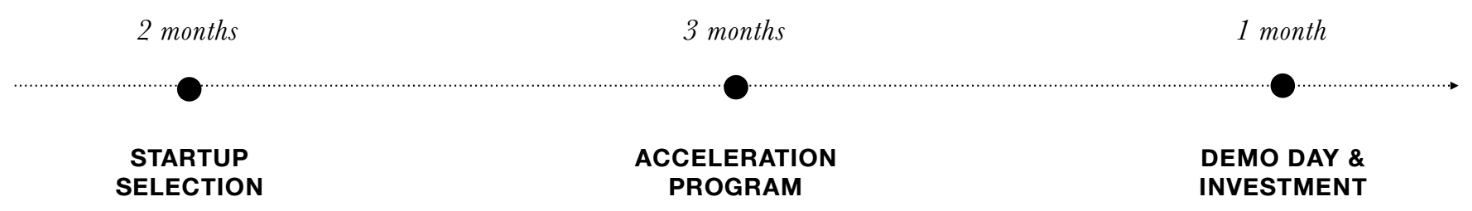
\includegraphics[height=2cm]{hcamp_resume}
\caption{Distribuzione temporale delle fasi previste dal programma H-CAMP}
\end{center}
\end{figure}

\subsection{Secondo pilastro: industria}
Le nuove tendenze tecnologiche dei consumatori obbligano le aziende a rivalutare le modalità con le quali investono sul personale, sui processi e sulle tecnologie. H-FARM aiuta la aziende a trasformare i loro modelli d'impresa e le loro attività in armonia con i cambiamenti digitali in atto.
\\ \\
La strategia per l’industria propone:
\begin{itemize}
\item \textbf{Digital transformation}: formazione, innovazione e rinnovamento dei processi organizzativi per diventare protagonisti del cambiamento digitale in ambito aziendale;
\item \textbf{H-ACK}: maratone di 24 ore focalizzate su specifici settori del'’industria. I partecipanti si dividono in team e lavorano per trovare soluzioni a problemi concreti esposti dalla compagnia promotrice dell'evento.
\end{itemize}

\subsection{Terzo pilastro: istruzione}
I tradizionali sistemi educativi stanno rapidamente diventando obsoleti e la domanda di metodi di apprendimento innovativi è in rapida crescita. H-FARM è il più grande ecosistema digitale attualmente presente in Italia, che unisce le best practice del mondo accademico con nuovi metodi di apprendimento presi in prestito dal mondo del business e delle \gls{startupg}\glsfirstoccur.
\\ \\
Per Maggio 2017 è prevista l'inaugurazione di una nuova area dedicata ad H-CAMPUS: il nuovo progetto formativo di H-FARM dedicato alla diffusione della cultura digitale attraverso un approccio innovativo. 
Studenti, professionisti e manager saranno accompagnati e resi protagonisti del processo di trasformazione digitale.
H-CAMPUS nascerà all'interno di un grande spazio aperto che andrà ad ospitare una \gls{internationalschool}\glsfirstoccur{} (dai 6 ai 18 anni) ed una università con più di 20 tra insegnanti e formatori.

\begin{figure}[htbp]
\begin{center}
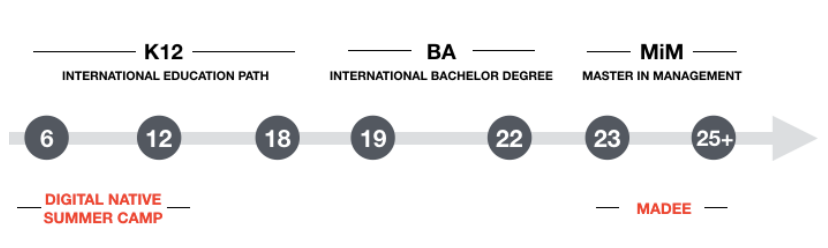
\includegraphics[height=4cm]{hfarm_education_graph}
\caption{Programma H-CAMPUS rivolto a diverse fasce d'età}
\end{center}
\end{figure}

%**************************************************************
\section{Digital Accademia}
Digital Accademia è il centro italiano di riferimento per la diffusione della cultura digitale ed è  situata all'interno dell'ecosistema H-FARM. \\
Questo è il luogo dove studenti, professionisti e innovatori possono conoscere il potenziale del digitale, integrarlo nei propri processi di sviluppo e guardare al futuro. Il tutto viene veicolato attraverso un approccio concreto, con il quale si mira alla formazione attraverso l'esperienza.
\\ \\
L'offerta di Digital Accademia si rivolge principalmente alle aziende e propone strumenti di gestione della conoscenza, strumenti di comunicazione e sessioni formative che consentano di rimanere al passo con il cambiamento costante. La cultura digitale offre possibilità di interazione impensabili fino a poco tempo fa e permette di veicolare contenuti in modo nuovo, coinvolgente, personale e non convenzionale.

\begin{figure}[htbp]
\begin{center}

\includegraphics[height=3cm]{logos/da_logo}
\caption{Logo Digital Accademia}
\end{center}
\end{figure}

\subsection{Formazione}
Diffondere la cultura digitale in azienda significa prima di tutto venire in contatto con le persone e con le loro competenze. L'innovazione del digitale non è un concetto astratto
ma una prassi, per questo non bastano corsi di aggiornamento o sessioni di formazione in aula. 
La formazione deve essere, prima di tutto, un'esperienza che coinvolge. 

\subsubsection{Bootcamp}
All'interno dell'offerta di formazione si colloca il progetto \textbf{Bootcamp}: un'esperienza full immersion di 3 giorni e 3 notti sulla cultura digitale, ospitata in Villa Annia: il quartier generale di Digital Accademia.
\\ \\
Le giornate alternano momenti di teoria a sessioni di pura pratica, mentre i pranzi, le cene e le sere sono momenti sempre conviviali arricchiti dalla presenza di ospiti ed esperti del settore di pertinenza per: 
\begin{itemize}
\item Imparare a pensare digitale;
\item Capire come funziona una buona storia;
\item Scoprire le logiche dietro a un e-commerce di successo; 
\item Costruire presentazioni persuasive.
\end{itemize}

\subsection{Comunicazione interna}
Le esperienze di comunicazione interna più efficaci parlano ai dipendenti come si parlerebbe al pubblico di un evento di \textit{entertainment}. 
L’avvento massiccio del digitale ha fatto sì che non ci sia più differenza tra comunicazione esterna ed interna all’azienda.

\subsubsection{Plot}
All'interno dell'offerta per la comunicazione interna si colloca il progetto \textbf{Plot}.
\\ \\
Questo progetto si basa sui principi degli \gls{arg}\glsfirstoccur{} per coinvolgere e divertire le persone all'interno di una organizzazione. I dipendenti si trasformano in giocatori e partecipano alla risoluzione di enigmi come in un romanzo giallo interattivo: analizzando i file aziendali e individuando informazioni nel mondo reale devono riuscire ad arrivare alla soluzione.
\\ \\
Pensato inizialmente per Vodafone, Plot è un'esperienza avvincente progettata per coinvolgere gli impiegati di tutto il mondo in un gioco mirato a salvare una loro collega, Sugita, rapita da un'intelligenza artificiale da essa stessa progettata.
\\ \\
Sugita rivela ai partecipanti di aver lasciato alcune \textit{backdoor} durante la fase di testing dell'intelligenza artificiale, ogni backdoor richiede una password che può essere trovata da qualche parte all'interno della intranet Vodafone. 
Per trovare le password, i giocatori (divisi in gruppi) devono studiare prodotti specifici dell'azienda, guardare tutorial e interagire tra loro e con i sistemi interni.
\\ \\
Sono previsti dieci livelli e dieci settimane di gioco, durante le quali i team provenienti da tutto il mondo si sfidano per salvare Sugita.
\\ \\
Terminati i dieci livelli, è prevista un'ultima fase nella quale le migliori squadre da tutto il mondo si sfidano a Londra in un'intensa giornata di gioco.
\\ \\
La squadra vincitrice si aggiudica le 6.000 sterline messe in palio come ricompensa.
\\ \\
Il Plot sviluppato per Vodafone ha registrato un grande successo, con oltre 8.000 giocatori distribuiti in 21 paesi. Questo ha portato a riproporre il format per altri clienti, tra i quali TUI Group e Assicurazioni Generali. 

\paragraph{La struttura}
Perchè abbia successo, il gioco non deve essere presentato come tale ma deve confondersi quanto più possibile con la realtà degli eventi. A questo scopo, la presentazione deve avvenire all'interno del contesto lavorativo. Ad esempio, nel caso di Vodafone, il meeting annuale dei dipendenti veniva interrotto da un video nel quale l'intelligenza artificiale comunicava di aver rapito Sugita e sfidava i colleghi a salvarla.
\\ \\
Dopo aver effettuato la registrazione presso il sistema, la piattaforma prevede una \textbf{fase di inviti} durante la quale ogni utente può invitare un certo numero di colleghi a far parte della propria squadra.
\\ \\
Al termine di questa fase, un algoritmo si occupa di formare le squadre secondo le preferenze espresse dagli utenti. Idealmente, se l'utente A sceglie l’utente B e l’utente B accetta, gli utenti A e B vengono inseriti nella stessa squadra.
\\ \\
Una volta chiusa la fase di inviti e formate le squadre, inizia la \textbf{fase di gioco}. 
La fase di gioco si articola in varie \textbf{mission}, ognuna può essere pensata come un blog che, durante la settimana, viene popolato tramite \textbf{post} appartenenti a tre possibili tipologie: 
\begin{itemize}
	\item \textbf{Testo}: introduce, in modo molto generale, l’obiettivo della mission e può avere contenuti multimediali come immagini e video;
	\item \textbf{Captcha}: prevede una domanda rivolta singolarmente all'utente, atta a verificare che esso sia effettivamente un umano e non una macchina;
	\item \textbf{Team}: prevede una domanda rivolta alla squadra. 
\end{itemize}

In questa fase, ogni settimana prevede due momenti chiave:
\begin{itemize}
	\item Ogni \textbf{lunedì} viene pubblicata una nuova mission, alla quale sono associati inizialmente un post di tipo testo e un post di tipo captcha;
	\item Ogni \textbf{mercoledì} viene pubblicato un post di tipo team, associato alla mission del lunedì.
\end{itemize}

\begin{figure}[htbp]
\begin{center}
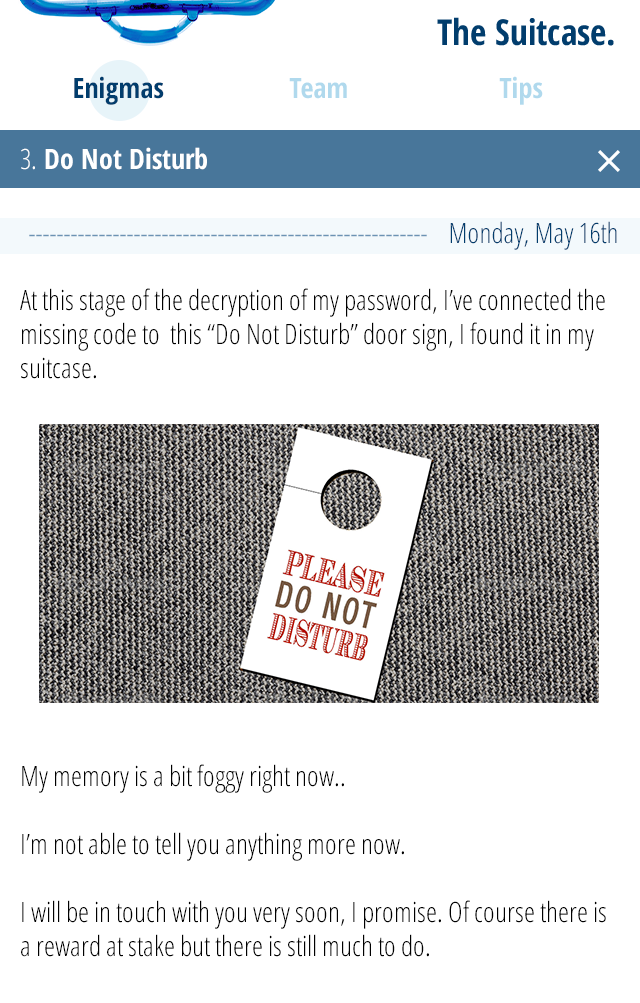
\includegraphics[height=9cm]{plot/text_post}
\caption{Un post di tipo testo}
\end{center}
\end{figure}

\begin{figure}[htbp]
\begin{center}
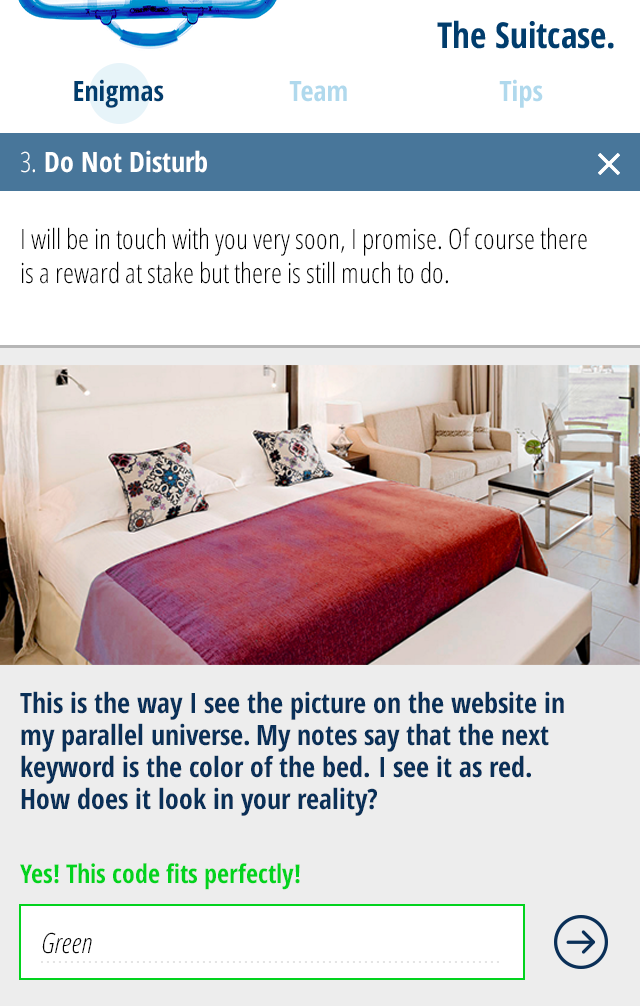
\includegraphics[height=9cm]{plot/captcha_post}
\caption{Un post di tipo captcha}
\end{center}
\end{figure}

\begin{figure}[htbp]
\begin{center}
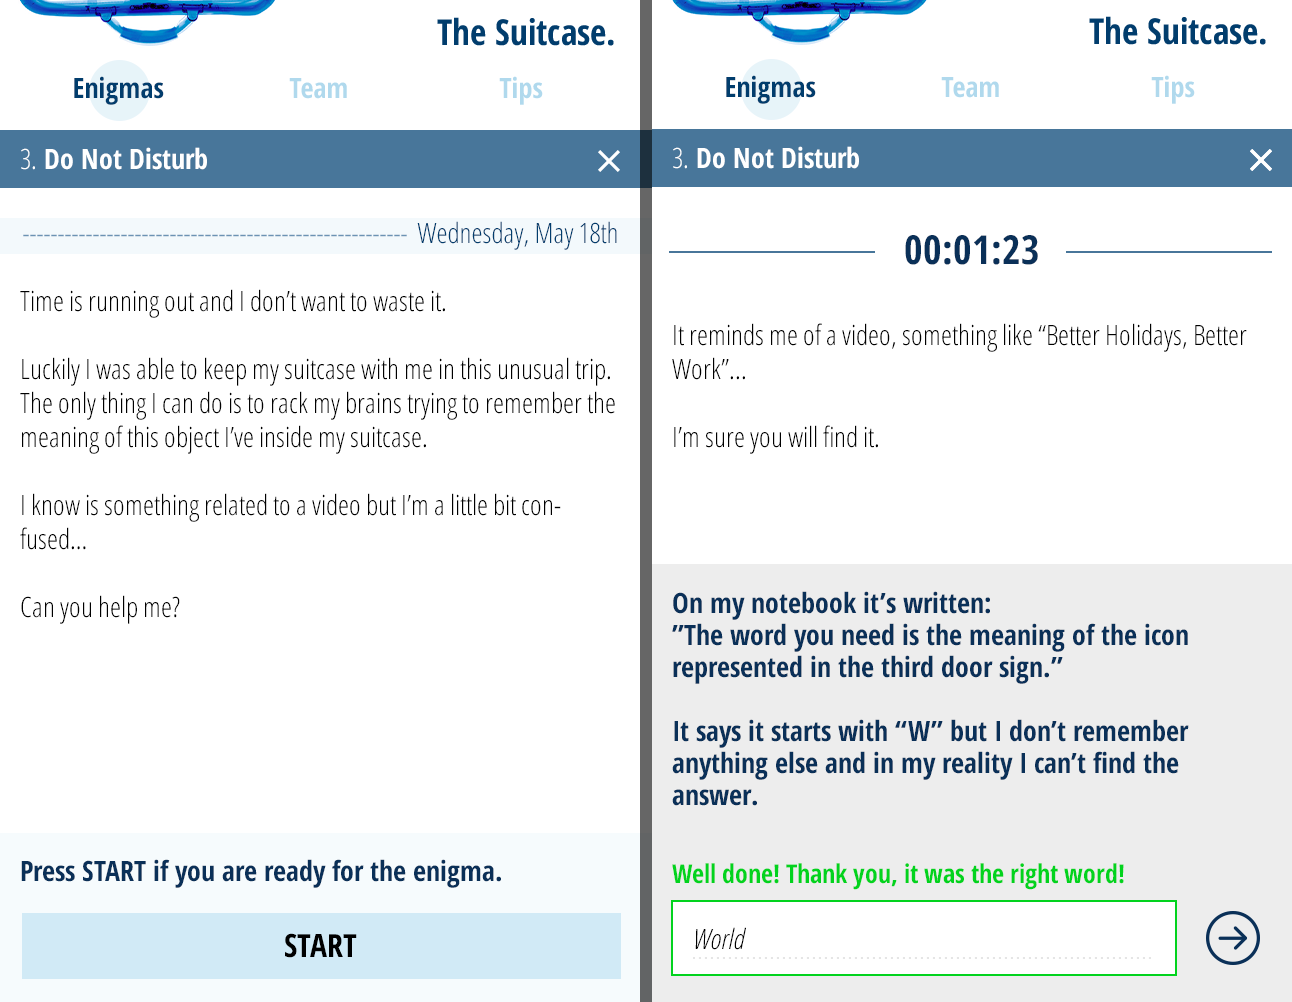
\includegraphics[height=9cm]{plot/team_post}
\caption{Un post di tipo team}
\end{center}
\end{figure}

Per accedere al post di tipo team è necessario che almeno la metà dei componenti della squadra abbia risposto alla propria domanda di tipo captcha. 
\\ \\
Le domande di tipo captcha sono uniche rispetto all'utente e alla squadra, con questo si intende che una specifica domanda di tipo captcha:
\begin{itemize}
	\item non viene presentata allo stesso utente più di una volta;
	\item non viene presentata ai compagni di squadra.
\end{itemize}

La domanda associata al post di tipo team non è immediatamente visibile alla pubblicazione del post, ma può essere svelata da un componente della squadra. Una volta svelata la domanda di tipo team, viene avviato un cronometro che registra il tempo impiegato dalla squadra per rispondere.
\\ \\
Mentre le domande di tipo captcha sono pensate per richiedere uno sforzo minimo all’utente, quelle di tipo team hanno grado di difficoltà più alto, che aumenta col progredire del gioco.
\\ \\
Le domande sono pensate in modo da portare gli utenti ad affrontare specifici \textbf{touchpoint}: strumenti o concetti che l'azienda vuole far conoscere ai propri dipendenti. \\
Ad esempio, nel caso di Vodafone, Plot è stato progettato per perseguire i seguenti touchpoint:
\begin{itemize}
	\item Far conoscere ai dipendenti di tutto il mondo una nuova area della intranet aziendale;
	\item Creare coesione tra i dipendenti;
	\item Attivare forme di coinvolgimento dirette attraverso la costruzione di un'esperienza;
	\item Trovare nuovi strumenti globali di comunicazione interna.
\end{itemize}

La squadra riceve un punteggio per ogni mission e, tale punteggio, è una funzione del tempo impiegato per rispondere alla domanda di tipo team. \\
Il punteggio totale di una squadra, che determina la posizione in classifica della stessa, è ricavato come somma dei punteggi ottenuti nelle varie mission.
             % Contesto aziendale
% !TEX encoding = UTF-8
% !TEX TS-program = pdflatex
% !TEX root = ../tesi.tex
% !TEX spellcheck = it-IT

%**************************************************************
\chapter{Il progetto di stage}
\label{cap:progetto-stage}

%**************************************************************
\section{Il contesto}
\label{sec:contesto}
La piattaforma Plot è composta da due moduli Laravel distinti: un modulo di gioco ed un modulo \gls{cms}\glsfirstoccur.
\\ \\
Il \textbf{modulo di gioco} incorpora la logica necessaria all'utente per interagire con la piattaforma. Questo modulo permette quindi agli utenti finali di:
\begin{itemize}
	\item Autenticarsi;
	\item Invitare altri utenti a far parte della propria squadra;
	\item Accedere al contenuto delle mission;
	\item Accedere al contenuto dei post;
	\item Accedere e rispondere alle question che vengono loro proposte;
	\item Accedere alle informazioni riguardanti il proprio team;
	\item Consultare la classifica generale.
\end{itemize}

Il \textbf{modulo \gls{cms}\glsfirstoccur{}} incorpora la logica necessaria agli amministratori per gestire il Plot. Questo modulo permette quindi agli amministratori di:
\begin{itemize}
	\item Autenticarsi;
	\item Creare nuove mission;
	\item Eliminare mission esistenti;
	\item Modificare i dettagli di una particolare mission;
	\item Accedere all'elenco di tutte le mission;
	\item Creare nuovi post per una particolare mission;
	\item Eliminare post esistenti;
	\item Modificare i dettagli di un particolare post;
	\item Accedere all'elenco di tutti i post relativi ad una particolare mission;
	\item Creare nuove question per un particolare post;
	\item Eliminare question esistenti;
	\item Modificare i dettagli di una particolare question;
	\item Accedere all'elenco di tutte le question relative ad un particolare post;
	\item Accedere all'elenco degli utenti iscritti alla piattaforma;
	\item Eliminare utenti esistenti;
	\item Modificare i dettagli di un particolare utente;
	\item Accedere all'elenco dei compagni di team di un particolare utente;
	\item Accedere all'elenco dei team;
	\item Eliminare team esistenti;
	\item Modificare i dettagli di un particolare team;
	\item Accedere all'elenco dei componenti di un particolare team;
	\item Accedere alla classifica generale;
	\item Accedere all'elenco delle domande previste, corredate delle risposte corrette  e del tipo di post al quale sono associate;
	\item Accedere all'elenco delle risposte fornite dagli utenti.
\end{itemize}

Entrambi i moduli Laravel utilizzano il medesimo database MySQL per la persistenza dei dati (Figura~\ref{fig:coupled}). 
Il database, pensato inizialmente per Vodafone, è stato adattato per diversi Plot, modificandolo di volta in volta. Le continue modifiche hanno portato ad avere un database inconsistente e poco manutenibile, a causa anche della scarsa documentazione.
\\ \\
Ogni modulo Laravel prevede un \gls{frontend}\glsfirstoccur{} collegato ad un relativo \gls{backend}\glsfirstoccur{}. Le logiche che sottendono i due \gls{backend}\glsfirstoccur{} sono, però, molto simili e questo porta ad avere codice duplicato e poco manutenibile.
\\ \\
Ulteriori problematiche nascono dal fatto che entrambi i \gls{frontend}\glsfirstoccur{} sono fortemente accoppiati al relativo \gls{backend}\glsfirstoccur{}, questo implica una struttura poco modulare e difficilmente riusabile.
\\ \\
Nel prosieguo della trattazione, con l’appellativo “Plot 1.0” mi riferirò alla configurazione della piattaforma esistente prima dell'inizio del progetto di stage.

\begin{figure}[htbp]
\begin{center}
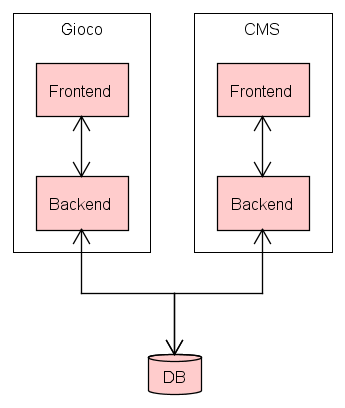
\includegraphics[height=8cm]{coupled-diagram}
\caption{Organizzazione della piattaforma prima del progetto di stage}
\label{fig:coupled}
\end{center}
\end{figure}

%**************************************************************
\section{Descrizione del progetto}
Il progetto di stage prevede tre attività principali:
\begin{enumerate}
	\item Refactoring del database che consente la persistenza dei dati utili alla piattaforma Plot;
	\item Creazione di un set di API REST che permettano di interagire con il database (di cui al punto 1);
	\item Refactoring del \gls{frontend}\glsfirstoccur{} relativo al \gls{cms}\glsfirstoccur.
\end{enumerate}

La piattaforma Plot è in continua evoluzione e mira ad adattarsi, quanto più possibile, alle richieste dei clienti. Le attività di progetto devono quindi essere affrontate con l'obiettivo di massimizzare la modularizzazione, in modo da consentire una buona manutenibilità della piattaforma ed un basso accoppiamento tra le parti.
\\ \\
Dato il respiro internazionale e multinazionale dei potenziali clienti della piattaforma, deve essere implementato il concetto di \textbf{traducibilità}: ogni risorsa di testo importante ai fini del gioco deve poter essere localizzata in base alla lingua preferita dall'utente che ne usufruisce.
\\ \\
Mantenere uno storico delle azioni effettuate dai giocatori può risultare utile per individuare la causa di eventuali problemi inaspettati, si richiede quindi di prevedere un meccanismo di \textbf{logging} che registri e renda accessibili le richieste HTTP effettuate dai giocatori.
\\ \\
Il set di API REST ed il \gls{frontend}\glsfirstoccur{} del \gls{cms}\glsfirstoccur{} dovranno consentire di effettuare tutte le operazioni già disponibili dall'interfaccia grafica del \gls{cms}\glsfirstoccur{} di Plot 1.0 (elencate nella sezione "`\hyperref[sec:hello]{Il contesto}"`). 
In aggiunta alle operazioni già note, dovrà essere possibile:
\begin{itemize}
	\item Accedere all'elenco degli amministratori della piattaforma;
	\item Eliminare gli amministratori;
	\item Modificare i dettagli di un particolare amministratore;
	\item Accedere all'elenco dei log generati dagli utenti del \gls{frontend}\glsfirstoccur{} di gioco;
	\item Accedere all'elenco delle traduzioni disponibili per una data risorsa;
	\item Eliminare le traduzioni relative ad una data risorsa;
	\item Modificare i dettagli di un particolare traduzione.
\end{itemize}

Non è richiesta un'interfaccia grafica professionale per il modulo \gls{cms}\glsfirstoccur{}.

%**************************************************************
\section{Tecnologie utilizzate}
\subsection{Database}
Per gestire il database è stato scelto \textbf{MySQL Workbench}: uno strumento di amministrazione visuale che permette di creare e modificare agevolmente lo schema di un database MySQL.
\\ \\
La scelta è ricaduta su questo strumento in quanto: 
\begin{itemize}
	\item Ufficialmente supportato e consigliato dalla comunità MySQL;
	\item Fornisce un procedimento assistito per la creazione dello schema, facilitando l'individuazione di errori.
\end{itemize}

\begin{figure}[htbp]
\begin{center}

\includegraphics[height=2cm]{logos/mysql-workbench-logo}
\caption{Logo MySQL Workbench}
\end{center}
\end{figure}

\subsection{Framework}
\subsubsection{Back end}
Il framework principale utilizzato per il progetto è \textbf{Laravel}: un framework PHP open-source, pensato per la creazione di applicazioni web basate sul pattern architetturale MVC (Model-View-Controller). 
\\ \\
Il framework è stato scelto dall'azienda per i vantaggi che offre, tra i quali:
\begin{itemize}
	\item Una documentazione ampia e facilmente consultabile in rete;
	\item Una sintassi pulita ed intuitiva;
	\item Facilità di implementazione della dependency injection;
	\item \textit{Eloquent}: \gls{orm}\glsfirstoccur{} integrato di Laravel;
	\item \textit{Blade}: il template engine integrato di Laravel.
\end{itemize}

\begin{figure}[htbp]
\begin{center}

\includegraphics[height=2cm]{logos/laravel-logo-white}
\caption{Logo Laravel}
\end{center}
\end{figure}

\subsubsection{Front end}
Per il refactoring dell'interfaccia grafica del \gls{cms}\glsfirstoccur{} è stato utilizzato \textbf{Bootstrap}: un framework HTML, CSS e JavaScript per la creazione di pagine web responsive e mobile-first.
\\ \\
Il framework è stato scelto perchè:
\begin{itemize}
	\item Mette a disposizione tutti i componenti base e gli stili utili per la creazione di una pagina web (layout a griglia, tabelle, box modali, form e molto altro);
	\item Viene supportato da tutti i maggiori browser;
	\item Permette di creare interfacce grafiche consistenti, anche senza modificare le componenti fornite;
	\item Pensato per creare pagine responsive che si adattino anche ai dispositivi mobile;
	\item Include un set di icone pronte all'uso;
	\item Ha una buona documentazione ed un grande supporto dalla comunità;
	\item Esistono molti temi, template e plugin gratuiti.
\end{itemize}

Oltre ai molti pregi, questo framework porta con sé almeno due difetti: 
\begin{itemize}
	\item Produce codice HTML verboso che può risultare non perfettamente semantico;;
	\item Molti componenti non funzionano se JavaScript è disattivato.
\end{itemize}

In accordo con l'azienda, questi non sono stati ritenuti problemi bloccanti in quanto il \gls{cms}\glsfirstoccur{} verrà ospitato su un server privato e sarà ad uso esclusivo degli amministratori, che avranno cura di utilizzare un browser che supporti JavaScript.

\begin{figure}[htbp]
\begin{center}

\includegraphics[height=2cm]{logos/bootstrap-logo}
\caption{Logo Bootstrap}
\end{center}
\end{figure}

\subsection{Versionamento}
Per il versionamento del codice è stato è stato utilizzato \textbf{Bitbucket} con base \textbf{Git}, in quanto già in uso presso l'azienda.
Bitbucket è un servizio di web-hosting per progetti software che utilizzano Git o Mercurial come sistemi di versionamento.
\\ \\
Il punto di forza di Bitbucket è la possibilità di creare, gratuitamente, repository privati. Questo risulta fondamentale per un'azienda che voglia mantenere il codice dei propri progetti accessibile solo a determinate persone.

\begin{figure}[htbp]
\begin{center}

\includegraphics[height=2cm]{logos/Atlassian_Bitbucket_Logo}
\caption{Logo Bitbucket}
\end{center}
\end{figure}

Git è un software per il versionamento distribuito ed è stato scelto dall'azienda in quanto offre:
\begin{itemize}
	\item Semplicità di utilizzo;
	\item Una buona documentazione disponibile online;
	\item La possibilità di lavorare anche offline, in quanto ogni sviluppatore possiede una copia locale del repository sul quale può effettuare commit anche in assenza di connessione. 
\end{itemize} 

\begin{figure}[htbp]
\begin{center}

\includegraphics[height=1.5cm]{logos/git-logo}
\caption{Logo Git}
\end{center}
\end{figure}

\subsection{Gestione di progetto}
Per la gestione di progetto è stato è stato utilizzato \textbf{Basecamp}, in quanto già in uso presso l'azienda.
\\ \\
Basecamp è un servizio web per che permette di condividere e organizzare tutto ciò che è necessario per la gestione di un progetto: task, discussioni, deadline e file.

\begin{figure}[htbp]
\begin{center}

\includegraphics[height=1.5cm]{logos/Basecamp-logo}
\caption{Logo Basecamp}
\end{center}
\end{figure}             % Progetto di stage
% !TEX encoding = UTF-8
% !TEX TS-program = pdflatex
% !TEX root = ../tesi.tex
% !TEX spellcheck = it-IT

%**************************************************************
\chapter{Descrizione dello stage}
\label{cap:descrizione-stage}
%**************************************************************

\intro{Breve introduzione al capitolo}\\

%**************************************************************
\section{Introduzione al progetto}

%**************************************************************
\section{Analisi preventiva dei rischi}

Durante la fase di analisi iniziale sono stati individuati alcuni possibili rischi a cui si potrà andare incontro.
Si è quindi proceduto a elaborare delle possibili soluzioni per far fronte a tali rischi.\\

\begin{risk}{Performance del simulatore hardware}
    \riskdescription{le performance del simulatore hardware e la comunicazione con questo potrebbero risultare lenti o non abbastanza buoni da causare il fallimento dei test}
    \risksolution{coinvolgimento del responsabile a capo del progetto relativo il simulatore hardware}
    \label{risk:hardware-simulator} 
\end{risk}

%**************************************************************
\section{Requisiti e obiettivi}


%**************************************************************
\section{Pianificazione}             % Analisi dei requsiti
%% !TEX encoding = UTF-8
% !TEX TS-program = pdflatex
% !TEX root = ../tesi.tex
% !TEX spellcheck = it-IT

%**************************************************************
\chapter{Progettazione e codifica}
\label{cap:progettazione-codifica}
%**************************************************************
\section{Progettazione del database}
\label{sec:progettazione}
Dall'analisi dei requisiti del database è stato possibile ricavare lo schema del database da implementare. Nel presente documento non è possibile riportare completamente tale schema a causa delle sue grandi dimensioni, ne verranno dunque descritti e riportati i dettagli salienti. \bigskip

Per ottenere lo schema finale è stato innanzitutto modellato uno schema concettuale di base, tale schema è stato successivamente ristrutturato in modo da:

\begin{itemize}
	\item Eliminare le \gls{ridondanza}\glsfirstoccur{} non necessarie;
	\item Eliminare le gerarchie: \gls{mysql}\glsfirstoccur{} non consente la rappresentazione diretta di una gerarchia, si deve quindi trasformare tale costrutto in modo che possa essere implementato;
	\item Partizionare le relazioni N-N: tali relazioni sono da evitare in quanto portano ad avere valori duplicati in entrambe le entità che vi partecipano. La presenza di valori duplicati implica una maggiore complessità nella risoluzione delle query e, quindi, un abbassamento generale delle performance. Per ovviare a questo problema sono state introdotte varie \textit{entità aggregate} per dividere una relazione N-N in due relazioni 1-N o 0-N.
\end{itemize}

\subsection{Dizionario delle entità} %**************************
La tabella~\ref{tab:dizionario-entita} documenta il significato delle entità rappresentate nello schema finale del database, in modo da evitare quanto più possibile situazioni di ambiguità. \\

Ogni entità è dotata degli attributi: id, created\_at, updated\_at. Questi non sono stati riportati nel dizionario delle entità, in quanto sono stati messi in risalto solo gli attributi caratteristici di ogni entità.

\begin{longtabu} to \textwidth {l X[2] X}
	\toprule
	\textbf{Entità} & \textbf{Descrizione} & \textbf{Attributi}\\
	\midrule
	\endhead
	users                            & Utenti iscritti a solo scopo di gioco     & name,\par surname,\par email,\par password,\par remember\_token \\ \midrule
external\_auth                   & Token di autenticazione fornito da un servizio esterno                               & external\_uid                                                                             \\ \midrule
admins                           & Utenti con accesso al solo CMS                                                       & name,\par surname,\par email,\par password,\par remember\_token                                           \\ \midrule
invitations                      & Inviti mandati e ricevuti dagli utenti     &                                                                                           \\ \midrule
logs                             & Log generati dalle richieste HTTP effettuate dagli user nel gioco                    & method,\par url,\par user\_ip\_address,\par user\_agent,\par additional\_data                             \\ \midrule
regions                          & Aree geografiche previste dal gioco                                                  & name                                                                                      \\ \midrule
timezones                        & Fusi orari previsti dal gioco                                                        & code,\par name,\par offset                                                                        \\ \midrule
business\_roles                  & Ambiti lavorativi previsti dal gioco                                                 & name                                                                                      \\ \midrule
languages                        & Lingue supportate dal gioco                                                          & locale,\par code                                                                              \\ \midrule
translatable\_contents           & I contenuti traducibili del gioco, ovvero quei contenuti che possono essere tradotti & default\_text                                                                             \\ \midrule
translations                     & Tutte le traduzioni disponibili relativamente ai contenuti traducibili presenti nel gioco             & text                                                                                      \\ \midrule
teams                            & Squadre presenti nel gioco                                                           & name, cover\_image                                                                        \\ \midrule
missions                         & Mission previste dal gioco                                                           & cover\_image, is\_visible, start\_date, end\_date                                         \\ \midrule
text\_posts                      & I post di tipo testo                                                                 & is\_visible                                                                               \\ \midrule
captcha\_posts                   & I post di tipo captcha                                                               & is\_visible                                                                               \\ \midrule
team\_posts                      & I post di tipo team                                                                  & is\_visible,\par time\_limit                                                                  \\ \midrule
user\_questions                  & Domande rivolte ai singoli utenti                                                    &                                                                                           \\ \midrule
user\_correct\_answers           & Le risposte corrette previste per le domande rivolte ai singoli utenti                                & content                                                                                   \\ \midrule
user\_questions\_business\_roles & Associazione tra le domande rivolte ai singoli utenti e le aree lavorative alle quali sono indirizzate. In questo modo, ogni possibile user\_question può essere indirizzata a tutti quegli utenti aventi il medesimo business\_role       &                                                                                           \\ \midrule
made\_user\_questions            & Associazione tra gli utenti e le domande ad essi effettivamente rivolte              &                                                                                           \\ \midrule
user\_answers                    & Risposte fornite dagli utenti in merito alle domande ad essi effettivamente rivolte                      & content, is\_correct                                                                      \\ \midrule
team\_questions                  & Domande rivolte ai team                                                              &                                                                                           \\ \midrule
team\_correct\_answers           & Le risposte corrette previste per le domande rivolte ai team                                & content                                                                                   \\ \midrule
made\_team\_questions            & Associazione tra i team e le domande ad essi effettivamente rivolte                  &                                                                                           \\ \midrule
team\_answers                    & Risposte fornite dai team in merito alle domande ad essi effettivamente rivolte                      & content, is\_correct                                                                      \\ \midrule
scores                           & Punteggi ottenuti dai team nel completare le varie mission                           & points \\
	\bottomrule \\
	\caption{Dizionario delle entità} 
	\label{tab:dizionario-entita} \\
\end{longtabu}

\subsection{Dizionario delle relazioni} %**************************
La tabella~\ref{tab:dizionario-relazioni} documenta il significato delle relazioni rappresentate nello schema finale del database, in modo da evitare quanto più possibile situazioni di ambiguità. \\
La colonna "Entità" riporta le entità partecipanti alla relazione, accompagnate dalla loro cardinalità.

\begin{longtabu} to \textwidth {l X[2] X}
	\toprule
	\textbf{Relazione} & \textbf{Descrizione} & \textbf{Entità}\\
	\midrule
	\endhead
	have       & Associa un utente di gioco con il proprio token di autenticazione esterno            & users (0,1)\par external\_auth (1,1) \\ \midrule
do           & Associa un utente di gioco con gli inviti da esso spediti                            & users (0,N)\par invitations (1,1)   \\ \midrule
receive      & Associa un utente di gioco con gli inviti da esso ricevuti                           & users (0,N)\par invitations (1,1)   \\ \midrule
produce      & Associa un utente di gioco con i log prodotti dalle sue richieste HTTP               & users (0,N)\par logs (1,1)   \\ \midrule
belong      & Associa un utente di gioco con l'area geografica alla quale appartiene                & users (0,1)\par regions (0,N)   \\ \midrule
belong      & Associa un'area geografica con il fuso orario al quale appartiene                     & regions (1,1)\par timezones (0,N)   \\ \midrule
have      & Associa un utente di gioco con l'ambito lavorativo al quale appartiene                  & users (0,1)\par business\_roles (0,N)   \\ \midrule
speak      & Associa un utente di gioco alla sua lingua preferita                                   & users (1,1)\par languages (0,N)   \\ \midrule
address      & Associa ogni traduzione alla propria lingua                                          & translations (1,1)\par languages (0,N)   \\ \midrule
have         & Associa un contenuto traducibile con tutte le sue traduzioni disponibili             & translatable\_contents (0,N)\par translations (1,1)   \\ \midrule
have         & Associa un utente al team al quale appartiene                                        & users (0,1)\par teams (0,N)   \\ \midrule
name         & Associa una mission al contenuto traducibile che rappresenta il nome della mission stessa & missions (1,1)\par translatable\_contents (1,1)   \\ \midrule
have         & Associa un post di tipo testo con la mission alla quale appartiene                   & text\_posts (1,1)\par missions (0,N)   \\ \midrule
have         & Associa un post di tipo captcha con la mission alla quale appartiene                 & captcha\_posts (1,1)\par missions (0,N)   \\ \midrule
have         & Associa un post di tipo team con la mission alla quale appartiene                    & team\_posts (1,1)\par missions (0,N)   \\ \midrule
content      & Associa un post di tipo testo al contenuto traducibile che rappresenta il corpo del post stesso                  																																						& text\_posts (1,1)\par translatable\_contents (1,1)   \\ \midrule
abstract      & Associa un post di tipo captcha al contenuto traducibile che rappresenta il corpo del post stesso                  																																						& captcha\_posts (1,1)\par translatable\_contents (1,1)   \\ \midrule
abstract      & Associa un post di tipo team al contenuto traducibile che rappresenta il corpo del post stesso                  																																						& team\_posts (1,1)\par translatable\_contents (1,1)   \\ \midrule
choose        & Associa un post di tipo captcha al bacino delle domande che possono essere rivolte ai singoli utenti                																																						  & captcha\_posts (0,N)\par user\_questions (1,1)   \\ \midrule
choose        & Associa un post di tipo team al bacino delle domande che possono essere rivolte ai team                																																						     & team\_posts (0,N)\par team\_questions (1,1)   \\ \midrule
content       & Associa una domanda utente al contenuto traducibile che rappresenta il corpo della domanda stessa                  																																						& user\_questions (1,1)\par translatable\_contents (1,1)   \\ \midrule
content       & Associa una domanda di tipo team al contenuto traducibile che rappresenta il corpo della domanda stessa                  																																						& team\_questions (1,1)\par translatable\_contents (1,1)   \\ \midrule
have          & Associa una domanda utente alle risposte corrette previste per la domanda stessa	  & user\_questions (1,N)\par user\_correct\_answers (1,1)   \\ \midrule
aggregate     & Collega una associazione tra domanda utente e ambito lavorativo con la rispettiva domanda utente. Questa relazione nasce dalla scomposizione della relazione N-N che legava una domanda utente con gli ambiti lavorativi ai quali è rivolta	    & user\_questions\_business\_roles (1,1)\par user\_questions (0,N)\\ \midrule
aggregate     & Collega una associazione tra domanda utente e ambito lavorativo con il rispettivo ambito lavorativo. Questa relazione nasce dalla scomposizione della relazione N-N che legava una domanda utente con gli ambiti lavorativi ai quali è rivolta	    & user\_questions\_business\_roles (1,1)\par business\_roles (0,N)\\ \midrule
aggregate     & Collega una associazione tra domanda utente e l'utente al quale è stata rivolta con la rispettiva domanda utente. Questa relazione nasce dalla scomposizione della relazione N-N che legava una domanda utente con l'utente al quale è rivolta    & made\_user\_questions (1,1)\par user\_questions (0,N)\\ \midrule
aggregate     & Collega una associazione tra domanda utente e l'utente al quale è stata rivolta con l'utente stesso. Questa relazione nasce dalla scomposizione della relazione N-N che legava una domanda utente con l'utente al quale è rivolta    & made\_user\_questions (1,1)\par users (0,N)\\ \midrule
aggregate     & Collega una associazione tra domanda di tipo team e il team al quale è stata rivolta con la rispettiva domanda di tipo team. Questa relazione nasce dalla scomposizione della relazione N-N che legava una domanda di tipo team con il team al quale è rivolta    & made\_team\_questions (1,1)\par team\_questions (0,N)\\ \midrule
aggregate     & Collega una associazione tra domanda utente e l'utente al quale è stata rivolta con il team stesso. Questa relazione nasce dalla scomposizione della relazione N-N che legava una domanda di tipo team con il team al quale è rivolta    & made\_team\_questions (1,1)\par teams (0,N)\\ \midrule
refer     & Collega una associazione tra domanda utente e l'utente al quale è stata rivolta con le risposte fornite per tale domanda dall'utente coinvolto   & made\_user\_questions (0,N)\par user\_answers (1,1)\\ \midrule
refer     & Collega una associazione tra domanda di tipo team e il team al quale è stata rivolta con le risposte fornite per tale domanda dal team coinvolto   & made\_team\_questions (0,N)\par team\_answers (1,1)\\ \midrule
give     & Associa una risposta fornita per una domanda utente all'utente che l'ha effettivamente fornita   & user\_answers (1,1)\par users (0,N)\\ \midrule
give     & Associa una risposta fornita per una domanda di tipo team al team che l'ha effettivamente fornita   & team\_answers (1,1)\par teams (0,N)\\ \midrule
unveil     & Collega una associazione tra domanda di tipo team e il team al quale è stata rivolta con l'utente che ha svelato la domanda avviando il timer   & made\_team\_questions (0,1)\par users (0,N)\\ \midrule
have     & Associa un team ai punteggi ottenuti nella risoluzione delle varie mission   & teams (0,N)\par scores (1,1)\\ \midrule
have     & Associa un punteggio con la mission nella quale è stato ottenuto   & scores (1,1)\par missions (0,N)\\ 
	\bottomrule \\
	\caption{Dizionario delle relazioni} 
	\label{tab:dizionario-relazioni}\\
\end{longtabu}


\subsection{Regole di vincolo} %**************************
Alcuni vincoli e proprietà non sono immediatamente deducibili dallo schema del database, è stato quindi deciso di mettere per iscritto tali proprietà in modo da aumentare la chiarezza della progettazione:
\begin{enumerate}
	\item Ogni utente può inviare al più un invito a qualsiasi altro utente;
	\item Un utente può scegliere un'unica lingua preferita;
	\item Un utente può afferire al più ad ambito lavorativo;
	\item Un utente può appartenere al più un'area geografica;
	\item Uno punteggio deve appartenere ad un unico team e può riferirsi ad un'unica mission completata da tale team;
	\item Un post deve appartenere ad un'unica mission;
	\item Una domanda utente deve appartenere ad un unico post di tipo captcha;
	\item Una domanda di tipo team deve appartenere ad un unico post di tipo team;
	\item Una domanda di tipo team può essere svelata al più da un utente;
	\item Un'area geografica deve appartenere ad un unico fuso orario;
	\item Una risposta corretta deve riferirsi ad un'unica domanda;
	\item Una risposta deve riferirsi ad un'unica domanda;
	\item Un log deve riferirsi ad un unico utente;
	\item Una traduzione deve riferirsi ad un unico contenuto traducibile e ad un'unica lingua.
\end{enumerate}

%**************************************************************
\section{Progettazione ed implementazione del CMS}
\subsection{Descrizione dell'architettura}
Il framework Laravel agevola l'adozione del pattern architetturale \textbf{model-view-controller (MVC)}, che impone la suddivisione della \textit{business logic} dalla \textit{presentation logic}. Nelle applicazioni Laravel, la business logic coincide spesso con modelli di dati persistenti in un database mentre la presentation logic si concretizza in una serie di pagine web. \\
Il pattern MVC prevede tre componenti principali: \textbf{model}, \textbf{view} e \textbf{controller} (figura~\ref{fig:mvc}).

\begin{figure}
	\centering
  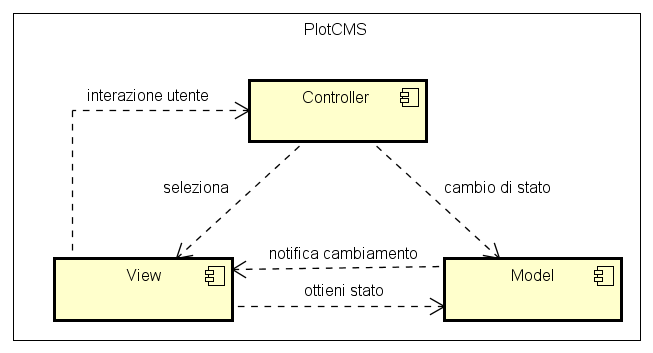
\includegraphics[scale=0.7]{immagini/components/mvc_diagram.png}
  \caption{Diagramma delle componenti del pattern MVC}
	\label{fig:mvc} 
\end{figure}

\subsubsection{Model} %****************************************************************
Il model rappresenta il dominio dell'applicazione e contiene l'astrazione di tutti i dati necessari al buon funzionamento della piattaforma. Nello specifico, esiste un'istanza di model per ogni entità prevista dal database collegato alla piattaforma, questo permette ed agevola l'interazione con il database attraverso l'\gls{orm}\glsfirstoccur{} Eloquent. \\
È compito del model notificare alla view eventuali cambiamenti avvenuti a livello del database, in modo da mostrare all'utente sempre e solo i dati aggiornati. \\
Le convenzioni del framework Laravel consigliano di posizionare le istanze del model nella directory \verb!app/Models!.

%**************************************************************************************

\subsubsection{View} %****************************************************************
La view è la rappresentazione visuale del model, cattura gli input dell'utente e ne delega l'elaborazione al controller. Nello specifico, l'interfaccia utente è composta da diverse pagine web che possono essere utilizzate dagli amministratori del \gls{cms}\glsfirstoccur{} per accedere alle varie funzionalità da esso offerte. \\
Le convenzioni del framework Laravel consigliano di posizionare le istanze della view nella directory \verb!resources/view!.

%**************************************************************************************

\subsubsection{Controller} %****************************************************************
Il controller coordina e crea un collegamento tra view e model, è responsabile quindi dell'elaborazione dell'input e dell'interazione con il model. \\
Le convenzioni del framework Laravel consigliano di posizionare le istanze del controller nella directory \verb!app/Http/Controllers!.

\begin{figure}
	\centering
  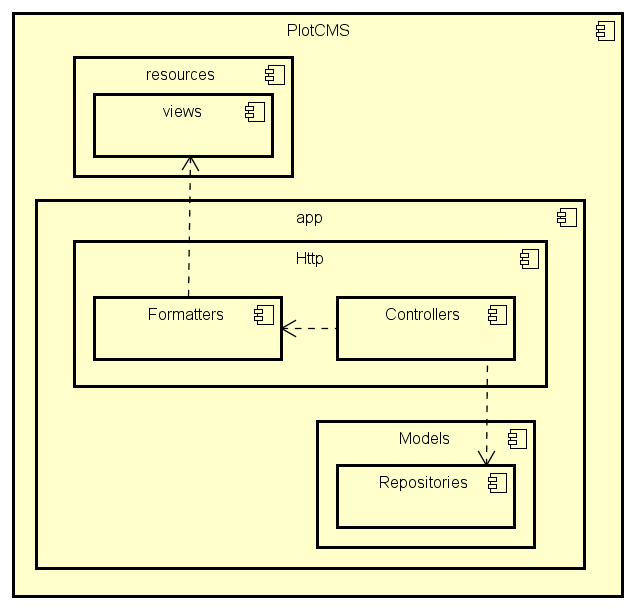
\includegraphics[scale=0.6]{immagini/components/important_components_diagram.png}
  \caption{Organizzazione delle principali componenti della piattaforma}
	\label{fig:components} 
\end{figure}

%**************************************************************
\section{Descrizione delle classi}
Di seguito sono descritte le classi e le interfacce più significative che compongono il \gls{cms}\glsfirstoccur{}, suddivise in base alla componente alla quale appartengono (le componenti fondanti del sistema sono riportate in figura~\ref{fig:components}). \\
Le classi appartenenti alla stessa componente hanno spesso implementazione simile in quanto, di base, permettono il compimento delle azioni \gls{crud}\glsfirstoccur{} su risorse di tipo diverso. Per evitare di appesantire la documentazione, è stato scelto di fornire un esempio di classe laddove la descrizione di tutte le classi avrebbe reso il testo fortemente ridondante. \\
Le classi appartenenti al framework sono state evidenziate in arancio nei diagrammi che le prevedono, in modo da poterle individuare facilmente.

\subsection{app::Models} %*******************************************************************************************

Le classi appartenenti a questa componente (figura~\ref{fig:models}) forniscono un'astrazione delle entità presenti nel database collegato alla piattaforma e sono utilizzate per interagire con esse. \\
L'\gls{orm}\glsfirstoccur{} \textit{Eloquent} richiede che tutti i model espongano particolari metodi utili a descrivere le relazioni esistenti tra le entità rappresentate dai model stessi a livello di database.

\begin{figure}[H]
	\centering
  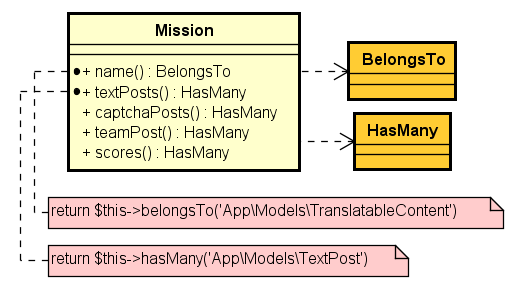
\includegraphics[scale=0.7]{immagini/components/mission.png}
  \caption{Diagramma della classe Mission}
	\label{fig:mission} 
\end{figure}

Ad esempio, la classe Mission (figura~\ref{fig:mission}) prevede i seguenti metodi:

\begin{itemize}
	\item \verb!name()!: rappresenta la relazione con cardinalità 1-1 tra una mission ed il contenuto traducibile che corrisponde al nome della mission stessa;
	\item \verb!textPosts()!: rappresenta la relazione con cardinalità 0-N tra una mission ed i post di tipo testo collegati alla stessa;
	\item \verb!captchaPosts()!: rappresenta la relazione con cardinalità 1-N tra una mission ed i post di captcha testo collegati alla stessa;
	\item \verb!teamPosts()!: rappresenta la relazione con cardinalità 1-N tra una mission ed i post di tipo team collegati alla stessa;
	\item \verb!scores()!: rappresenta la relazione con cardinalità 1-N tra una mission ed i punteggi totalizzati dai team relativamente alla mission stessa.
\end{itemize}

\begin{figure}[H]
	\centering
  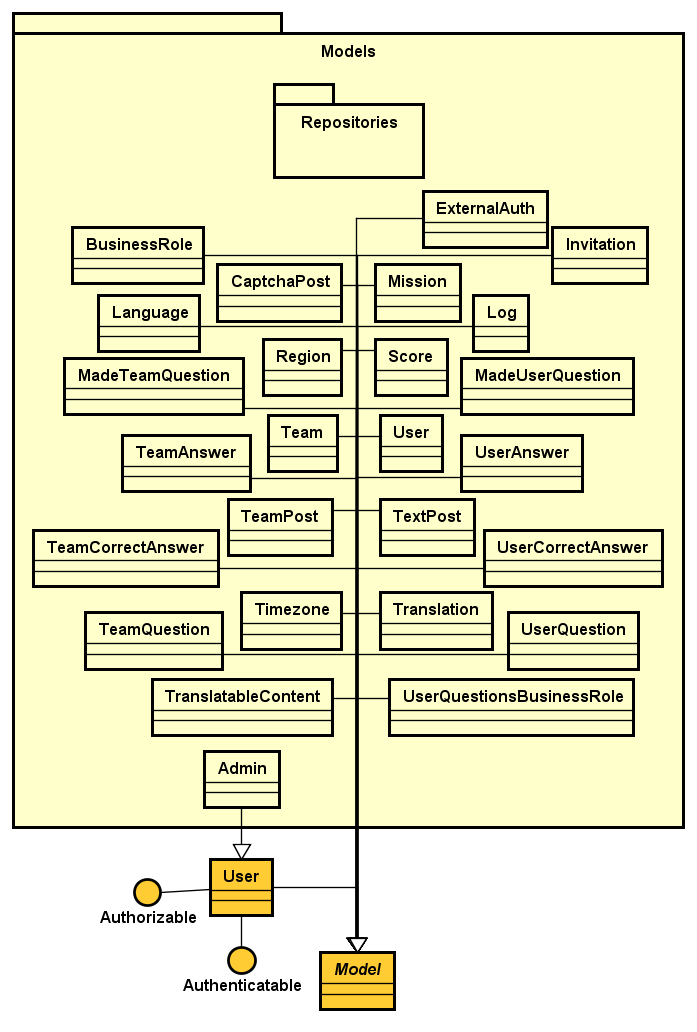
\includegraphics[scale=0.55]{immagini/components/models_diagram.png}
  \caption{Diagramma delle classi della componente Models}
	\label{fig:models} 
\end{figure}

Maggiori dettagli sui metodi esposti dall'\gls{orm}\glsfirstoccur{} Eloquent per rappresentare le relazioni tra model possono essere recuperati nella documentazione online ufficiale del framework Laravel (\cite{site:laravel-doc}).


\subsubsection{app::Models::Repositories} %*******************************************************************************************

\begin{figure}[H]
	\centering
  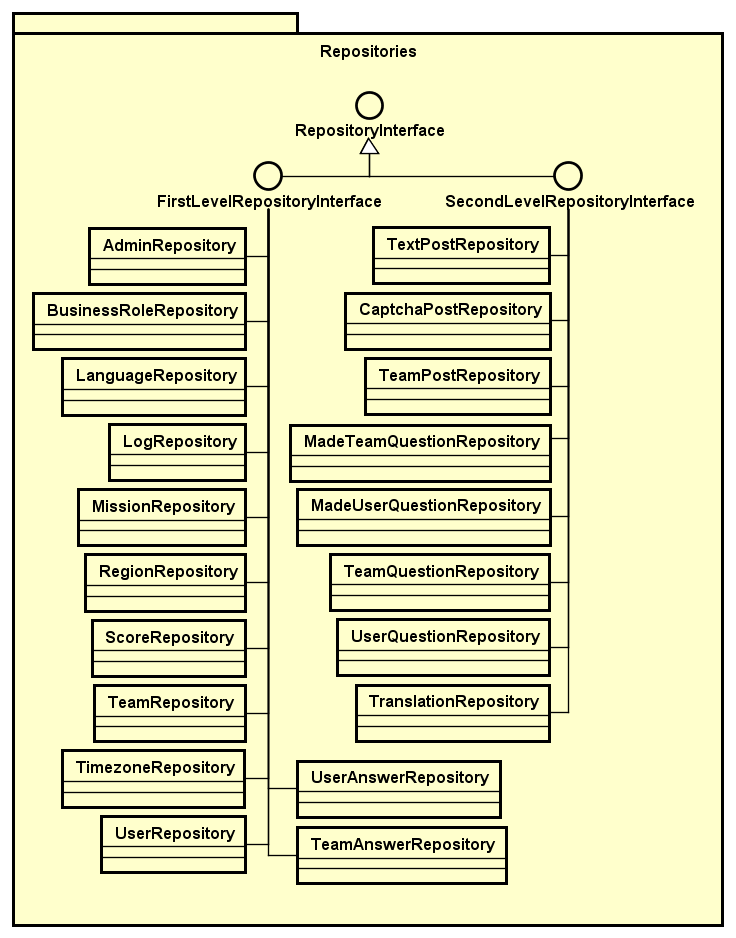
\includegraphics[scale=0.6]{immagini/components/repositories_diagram.png}
  \caption{Diagramma delle classi della componente Repositories}
	\label{fig:repositories} 
\end{figure}

Le classi e le interfacce appartenenti a questa componente (figura~\ref{fig:repositories}) sono utilizzate per implementare il design pattern \textbf{Repository}, utile per disaccoppiare la \textit{business logic} dal sistema di persistenza dati effettivamente utilizzato. In questo modo le istanze del controller possono effettuare query in modo dichiarativo sulle istanze del model, lasciando che siano i repository ad occuparsi dei dettagli implementativi delle query stesse. \\
Concettualmente, un repository incapsula l'insieme delle operazioni disponibili sulle entità di un database, così da fornire un modo più \textit{object-oriented} per accedervi.\bigskip

Le istanze di repository possono essere fondamentalmente di due tipi, in base al model che devono trattare:
\begin{itemize}
	\item \textbf{First level}: se l'istanza del repository è collegata ad un model la cui esistenza è autoesplicativa, ovvero non necessita di un secondo model; 
	\item \textbf{Second level}: se l'istanza del repository è collegata ad un model che ha senso di esistere solo come figlio di un secondo model. Un esempio di questa tipologia è TextPostRepository, collegato al model TextPost le cui istanze sono significative solo come figlie di un'istanza di Mission.
\end{itemize}

\begin{figure}[H]
	\centering
  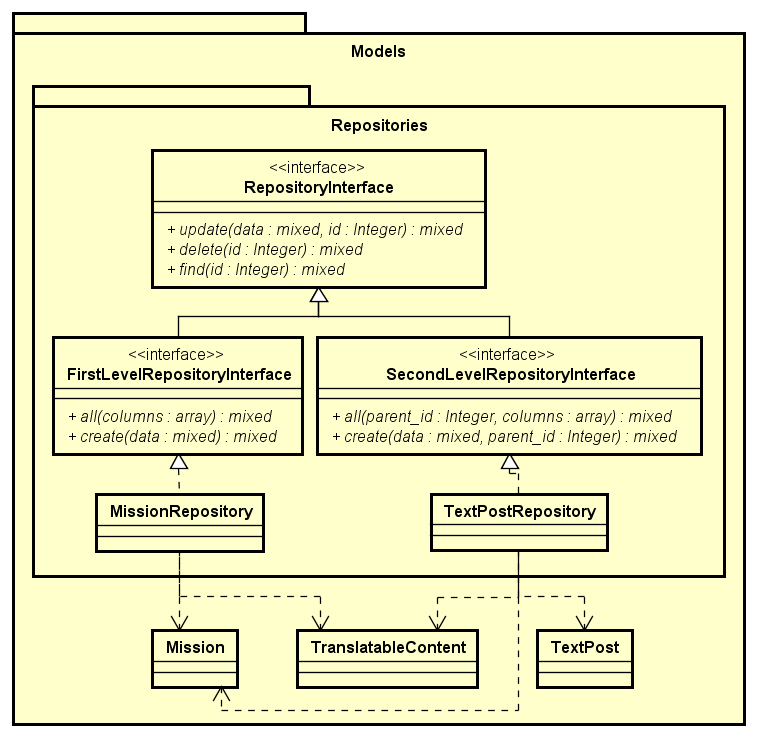
\includegraphics[scale=0.7]{immagini/components/repository_example.png}
  \caption{Diagramma delle classi MissionRepository e TextPostRepository}
	\label{fig:repository-example} 
\end{figure}

\newpage
Per modellare la situazione sopra descritta sono state usate delle interfacce:
\begin{itemize}
	\item \textbf{Repositories::RepositoryInterface}: espone metodi per effettuare l'aggiornamento, la rimozione o il recupero di particolari risorse. Tali metodi sono indipendenti dal tipo di repository;
	\item \textbf{Repositories::FirstLevelRepositoryInterface}: espone metodi per effettuare il recupero e la creazione di risorse che non prevedono una risorsa padre. Estende \verb!RepositoryInterface!;
	\item \textbf{Repositories::SecondLevelRepositoryInterface}: espone metodi per effettuare il recupero e la creazione di risorse che necessitano di una risorsa padre. Estende \verb!RepositoryInterface!.
\end{itemize}

In figura~\ref{fig:repository-example} sono riportati un esempio di repository \textit{first level} ed un esempio di repository \textit{second level}: MissionRepository e TextPostRepository. Il secondo differisce dal primo a causa del parametro \verb!parent_id!, necessario per individuare il padre della risorsa da creare e/o recuperare.

\subsection{resources::views} %******************************************************************************************

\begin{figure}[H]
	\centering
  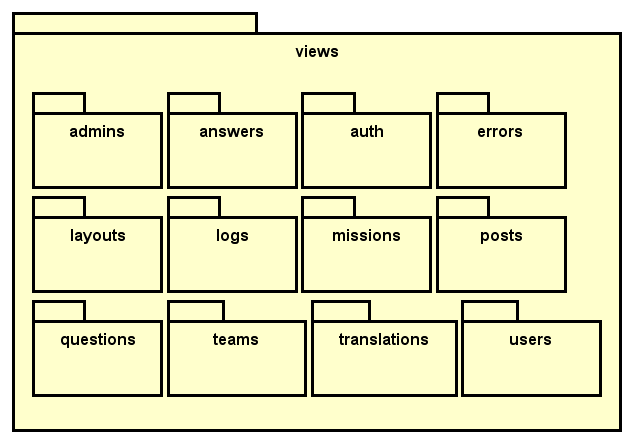
\includegraphics[scale=0.7]{immagini/components/views_diagram.png}
  \caption{Diagramma delle classi della componente views}
	\label{fig:views} 
\end{figure}

I file appartenenti a questa componente costituiscono l'interfaccia utente del \gls{cms}\glsfirstoccur{}, accessibile attraverso un browser web. L'interfaccia utente è stata ottenuta utilizzando i widget messi a disposizione dal template Bootstrap "Gentelella", liberamente disponibile online all'indirizzo \url{https://github.com/puikinsh/gentelella}. La scelta per la realizzazione dell'interfaccia utente è ricaduta sull'utilizzo di un template in modo da poter contenere i tempi di progettazione, senza dover per questo rinunciare alla qualità visiva e funzionale.\\

Per aumentare la modularizzazione delle view e la loro manutenibilità è stato utilizzato \textbf{Blade}: il \textit{template system} offerto dal framework Laravel. Grazie a Blade è possibile: 

\begin{itemize}
	\item Definire dei \textit{template} che fungano da base per la costruzione di diverse view;
	\item Utilizzare delle scorciatoie che agevolano azioni comunemente effettuate dalle view sui dati che devono mostrare, come stampare il valore di una variabile o scorrere una struttura dati.
\end{itemize}

L'utilizzo dei template ha reso possibile introdurre il concetto di ereditarietà, seppur abbastanza superficiale, nell'ambito HTML che ne è storicamente sprovvisto. \\
I file contenenti le view sono poi stati suddivisi sulla base del model al quale sono collegati (figura~\ref{fig:views}). Ad esempio, nella sotto-componente \textbf{views::missions} sono contenuti i file:

\begin{itemize}
	\item \textbf{all.blade}: struttura della view che mostra la lista di tutte le mission previste dal gioco;
	\item \textbf{create.blade}: struttura della view che presenta il form utile per creare una nuova mission;
	\item \textbf{edit.blade}: struttura della view che mostra il form utile a modificare i dettagli di una mission esistente;
	\item \textbf{show.blade}: struttura della view che mostra i dettagli di una mission esistente.
\end{itemize}

La sotto-componente più importante è \textbf{views::layouts} che contiene il file \textbf{app.blade}. Questo file definisce la base di ogni pagina web, una struttura a tre pannelli che prevede: 

\begin{itemize}
	\item Un menù di navigazione che riporta le sezioni più importanti del sito;
	\item Il nome dell'utente autenticato, associato alla possibilità di effettuare il logout;
	\item Il contenuto della pagina, provvisto dei dati richiesti dall'utente.
\end{itemize}

Tutte le view estendono \textbf{app.blade} in modo da mantenere un \textit{look-and-feel} consistente per l'intero sito.

\subsection{app::Http::Controllers} %*******************************************************************************************

Le classi e le interfacce appartenenti a questa componente (figura~\ref{fig:controllers}) sono deputate alla gestione delle richieste \gls{http}\glsfirstoccur{} in entrata: ogni richiesta viene inoltrata allo specifico controller in grado di soddisfarla. 
\\ \\
Nel framework Laravel, una \textit{route} rappresenta l'associazione tra una richiesta \gls{http}\glsfirstoccur{} e il controller utile alla sua risoluzione, tutte le route previste sono salvate nel file \verb!app/Http/routes.php!. 
Un esempio di route è il seguente:

\begin{lstlisting}[frame=none]
Route::get('missions.textposts','WebTextPostController@index')
\end{lstlisting}

Questa route indica che la piattaforma può gestire una richiesta \gls{http}\glsfirstoccur{} inoltrata all'\gls{url}\glsfirstoccur{} \verb!missions/mission_id/textposts/textpost_id! con metodo GET. La gestione è presa in carico dal metodo \verb!index! del controller \verb!WebTextPostController!. I segnaposto \verb!mission_id! e \verb!textpost_id! indicano che l'\gls{url}\glsfirstoccur{} prevede due parametri interi, positivi e non opzionali. Tali parametri rappresentano rispettivamente l'id del post di tipo testo che si vuole recuperare e l'id della mission alla quale il post è collegato. \\
Il passaggio dei parametri, contenuti nell'\gls{url}\glsfirstoccur{}, al metodo del controller viene completamente gestito dal framework Laravel: il primo parametro dell'\gls{url}\glsfirstoccur{} viene passato al primo parametro del metodo, il secondo parametro dell'\gls{url}\glsfirstoccur{} viene passato al secondo parametro del metodo e così via. 
Questa peculiarità implica che la struttura di ogni controller sia influenzata dal tipo di route che deve gestire, il tipo della particolare route dipende dal numero di parametri in essa presenti.\\ 
Sono stati quindi parametrizzati diversi tipi di controller:

\begin{itemize}
	\item \textbf{First level}: se il controller deve gestire una route con al più un parametro;
	\item \textbf{Second level}: se il controller deve gestire una route con al più due parametri;
	\item \textbf{Third level}: se il controller deve gestire una route con al più tre parametri;
	\item \textbf{Fourth level}: se il controller deve gestire una route con al più quattro parametri;
	\item \textbf{Fifth level}: se il controller deve gestire una route con al più cinque parametri.
\end{itemize}

Dall'analisi dei requisiti è emerso, inoltre, che la piattaforma deve essere accessibile sia attraverso un browser web sia attraverso le API REST esposte dalla stessa, sono stati quindi previsti due gruppi di route:

\begin{itemize}
	\item \textbf{Route web}: utilizzate per accedere all'interfaccia grafica del \gls{cms}\glsfirstoccur{} da browser web; 
	\item \textbf{Route API}: utilizzate per accedere alle API REST offerte dalla piattaforma. L'\gls{url}\glsfirstoccur{} per usufruire di una certa funzionalità attraverso una route API equivale all'\gls{url}\glsfirstoccur{} per accedere alla stessa funzionalità attraverso una route web, con l'aggiunta del prefisso \verb!api/v1!. Ad esempio, per accedere ad un'interfaccia grafica contenente la lista di tutte le mission è possibile utilizzare l'\gls{url}\glsfirstoccur{} \verb!/missions!, mentre per ottenere un pacchetto JSON contenente lo stesso risultato è possibile utilizzare l'\gls{url}\glsfirstoccur{} \verb!/api/v1/missions!.
\end{itemize}

La differenza tra i controller adibiti alla gestione delle route web e i controller adibiti alla gestione delle route API consiste nella sola formattazione del risultato restituito, questo ha portato all'utilizzo del design pattern \textbf{Template Method}. Il pattern Template Method permette di definire la struttura di un algoritmo lasciando alle sottoclassi il compito di implementarne alcuni passi, in questo modo è possibile ridefinire e personalizzare parte del comportamento nelle sottoclassi evitando codice duplicato. \\ 
La struttura dell'algoritmo è solitamente definita in un metodo chiamato \textit{template method}, tale metodo utilizza delle \textit{operazioni primitive} astratte che devono essere concretizzate dalle sottoclassi per specializzarne il comportamento. 

\begin{figure}[H]
	\centering
  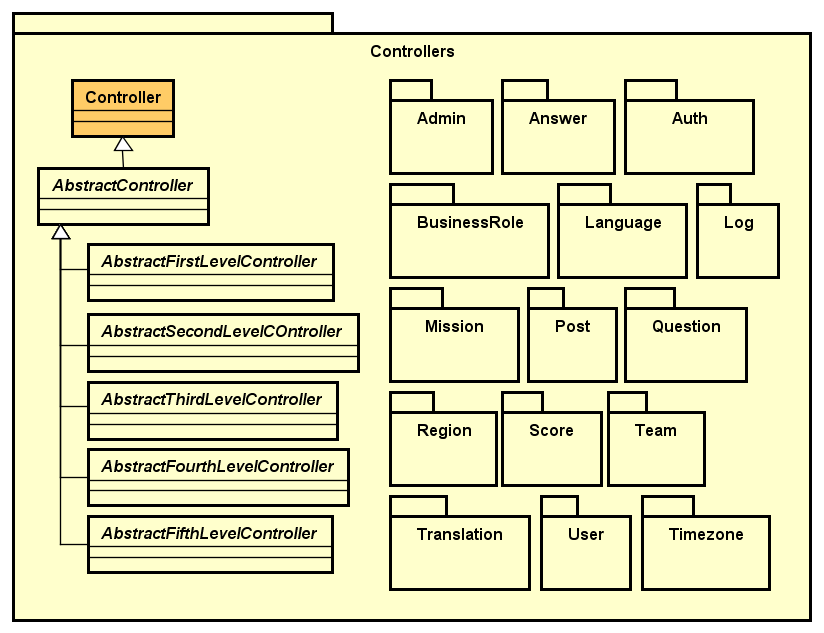
\includegraphics[scale=0.95, width=\textwidth]{immagini/components/controllers_diagram.png}
  \caption{Diagramma delle classi della componente Controllers}
	\label{fig:controllers} 
\end{figure}

Per modellare la situazione sopra descritta sono state utilizzate delle classi astratte:

\begin{itemize}
	\item \textbf{Controllers::AbstractController}: definisce l'attributo \verb!repository! che ospiterà il riferimento al principale repository utilizzato dalla classe che concretizza AbstractController. Per mantenere una struttura consistente, infatti, ogni controller non può accedere direttamente al model ma deve servirsi dell'apposito repository. Questa classe espone inoltre il metodo astratto \verb!format!, ovvero l'\textit{operazione primitiva} utilizzata dai metodi delle sottoclassi per restituire un risultato all'utente. Questo metodo deve essere implementato dalle sottoclassi in modo da restituire i dati nel formato corretto rispetto alla modalità d'accesso dell'utente alla piattaforma; 
	\item \textbf{Controllers::AbstractFirstLevelController}: definisce l'interfaccia dei controller di tipo \textit{first level};
	\item \textbf{Controllers::AbstractSecondLevelController}: definisce l'interfaccia dei controller di tipo \textit{second level};
	\item \textbf{Controllers::AbstractThirdLevelController}: definisce l'interfaccia dei controller di tipo \textit{third level};
	\item \textbf{Controllers::AbstractFourthLevelController}: definisce l'interfaccia dei controller di tipo \textit{fourth level};
	\item \textbf{Controllers::AbstractFifthLevelController}: definisce l'interfaccia dei controller di tipo \textit{fifth level}.
\end{itemize}

L'interfaccia dei controller è composta da una serie di metodi utili per: creare una nuova risorsa, recuperare una determinata risorsa, aggiornare una determinata risorsa, eliminare una determinata risorsa. \bigskip

\begin{figure}[H]
	\centering
  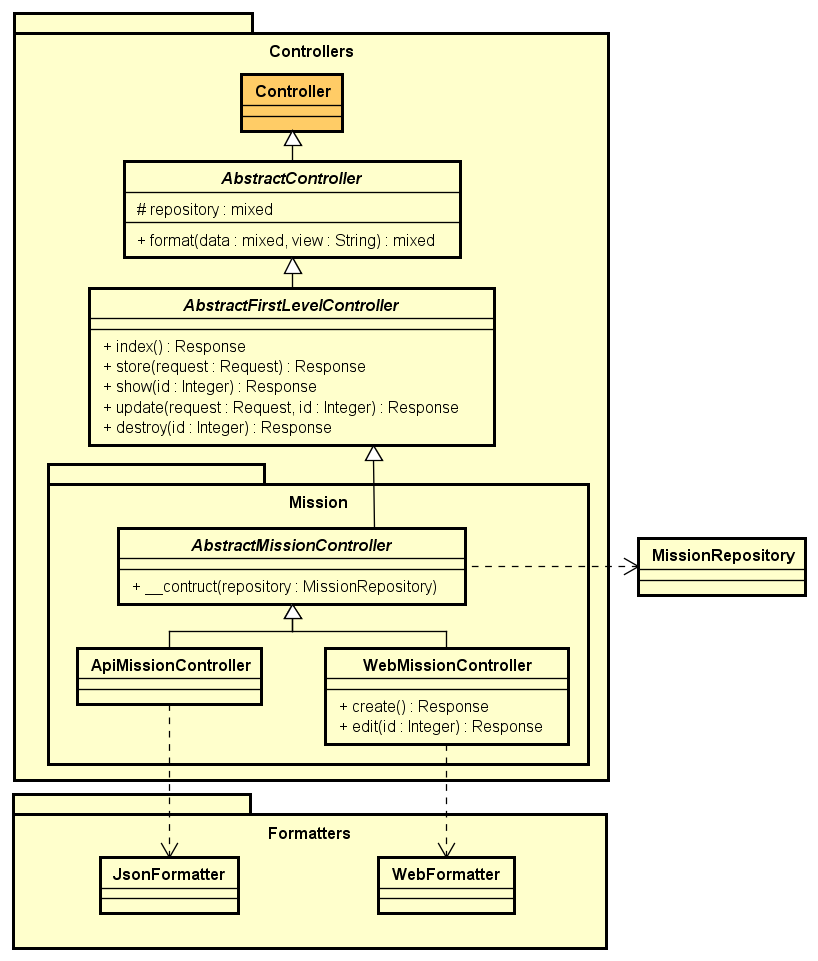
\includegraphics[scale=0.5, width=\textwidth]{immagini/components/controllers_example.png}
  \caption{Diagramma delle classi ApiMissionController e WebMissionController}
	\label{fig:controller-example} 
\end{figure}

Le classi appartenenti a questa componente adoperano il design pattern \textbf{Dependency Injection} per separare il loro comportamento dalla risoluzione delle dipendenze che espongono. In particolare questo pattern è utilizzato per \textit{iniettare}, utilizzando il costruttore della classe, le dipendenze relative ai repository usati da ogni controller.
 
Due esempi di controller di tipo \textit{first level} sono i controller adibiti alla gestione delle mission (figura~\ref{fig:controller-example}): ApiMissionController e WebMissionController. Questi controller derivano da \textbf{AbstractMissionController} che si occcupa di implementare i metodi ereditati da AbstractFirstLevelController. Le classi concrete \textbf{ApiMissionController} e \textbf{WebMissionController} hanno invece due compiti: 

\begin{itemize}
	\item Esporre eventuali metodi specifici e relativi ad una sola modalità di accesso, ad esempio i controller che gestiscono l'accesso tramite web (come WebMissionController) espongono metodi per mostrare i form utili alla creazione e aggiornamento delle risorse, questo non è necessario per i controller che gestiscono l'accesso tramite API (come ApiMissionController);
	\item Implementare il metodo astratto \verb!format!, utilizzando il costrutto appropriato della componente \hyperlink{formatters}{Formatters}.
\end{itemize} 

\hypertarget{formatters}{} %*******************************************************************************************
\subsection{app::Http::Formatters} 
\begin{figure}[H]
	\centering
  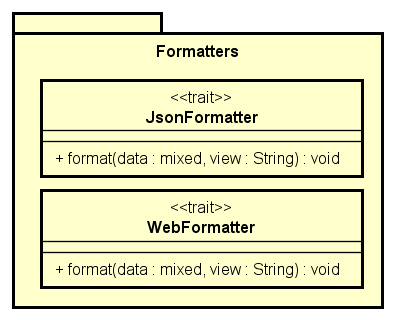
\includegraphics[scale=0.8]{immagini/components/formatters_diagram.png}
  \caption{Diagramma delle classi della componente Formatters}
	\label{fig:formatters} 
\end{figure}

La differenza fondamentale tra l'accesso tramite browser web e l'accesso tramite API REST riguarda la formattazione dei dati ottenuti come risultato della richiesta: 
\begin{itemize}
	\item Se l'accesso avviene tramite browser web, l'utente si aspetta di poter interagire con un'interfaccia grafica;
	\item Se l'accesso avviene tramite API REST, l'utente si aspetta di poter interagire con un formato di dati strutturato. In questo caso è stato scelto di fornire all'utente un pacchetto di dati in formato \gls{json}\glsfirstoccur{} in quando tale formato è oggi largamente utilizzato nello scambio di dati sul web, inoltre il framework Laravel ne rende molto agevole la manipolazione.
\end{itemize} 

Questa componente (figura~\ref{fig:formatters}) contiene due \gls{trait}\glsfirstoccur{} che si occupano proprio di formattare il risultato della richiesta in modo adeguato:
\begin{itemize}
	\item \textbf{Formatters::JsonFormatter}: restituisce i dati in formato \gls{json}\glsfirstoccur{};
	\item \textbf{Formatters::WebFormatter}: restituisce i dati attraverso una web view.
\end{itemize}

Entrambi i \gls{trait}\glsfirstoccur{} espongono un unico metodo: \verb!format!. Essi vanno intesi come dei pacchetti di codice pre-confezionato che agevolano lo sviluppatore nell'implementazione del metodo \verb!format! richiesto per la realizzazione di un controller concreto. In questo modo la scrittura di codice duplicato viene ridotta al minimo: lo sviluppatore deve solamente scegliere quale formatter utilizzare e non deve preoccuparsi di scrivere la procedura per la formattazione, in quanto questa è già incapsulata nel formatter scelto.




             % Concept Preview
%% !TEX encoding = UTF-8
% !TEX TS-program = pdflatex
% !TEX root = ../tesi.tex
% !TEX spellcheck = it-IT

%**************************************************************
\chapter{Progettazione e codifica}
\label{cap:progettazione-codifica}
%**************************************************************

\intro{Breve introduzione al capitolo}\\

%**************************************************************
\section{Tecnologie e strumenti}
\label{sec:tecnologie-strumenti}

Di seguito viene data una panoramica delle tecnologie e strumenti utilizzati.

\subsection*{Tecnologia 1}
Descrizione Tecnologia 1.

\subsection*{Tecnologia 2}
Descrizione Tecnologia 2

%**************************************************************
\section{Ciclo di vita del software}
\label{sec:ciclo-vita-software}

%**************************************************************
\section{Progettazione}
\label{sec:progettazione}

\subsubsection{Namespace 1} %**************************
Descrizione namespace 1.

\begin{namespacedesc}
    \classdesc{Classe 1}{Descrizione classe 1}
    \classdesc{Classe 2}{Descrizione classe 2}
\end{namespacedesc}


%**************************************************************
\section{Design Pattern utilizzati}

%**************************************************************
\section{Codifica}
             % Product Prototype
%% !TEX encoding = UTF-8
% !TEX TS-program = pdflatex
% !TEX root = ../tesi.tex
% !TEX spellcheck = it-IT

%**************************************************************
\chapter{Verifica e validazione}
\label{cap:verifica-validazione}
%**************************************************************             % Product Design Freeze e SOP
%% !TEX encoding = UTF-8
% !TEX TS-program = pdflatex
% !TEX root = ../tesi.tex
% !TEX spellcheck = it-IT

%**************************************************************
\chapter{Conclusioni}
\label{cap:conclusioni}
%**************************************************************

%**************************************************************
\section{Consuntivo finale}

%**************************************************************
\section{Raggiungimento degli obiettivi}

%**************************************************************
\section{Conoscenze acquisite}

%**************************************************************
\section{Valutazione personale}
             % Conclusioni
\appendix                               
%% !TEX encoding = UTF-8
% !TEX TS-program = pdflatex
% !TEX root = ../tesi.tex
% !TEX spellcheck = it-IT

%**************************************************************
\chapter{Casi d'uso secondari}
%**************************************************************

\hypertarget{UC3}{}
\section{Caso d'uso UC3: gestione user}

        \begin{figure}[H]
            \centering
            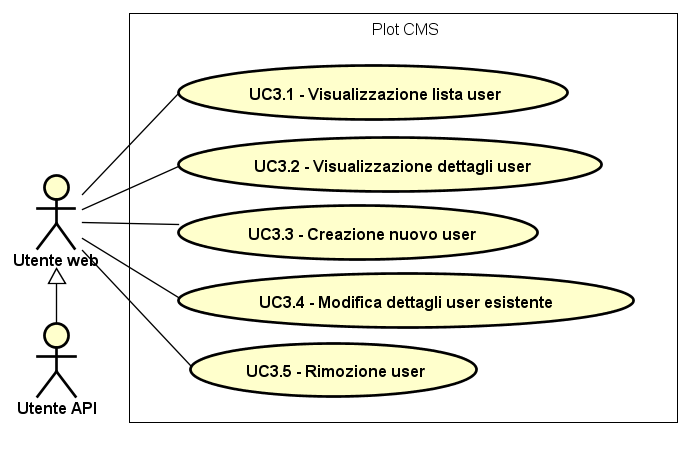
\includegraphics[scale=0.95, width=\textwidth]{immagini/usecase/UC3.png}
            \caption{Caso d'uso UC3: gestione user}\label{fig:UC3} 
        \end{figure}
\begin{itemize}
\item \textbf{Attori}: utente web, utente API;
\item \textbf{Descrizione}: un utente autenticato deve poter gestire gli aspetti di base legati agli utenti del gioco: creazione, visualizzazione, modifica e rimozione; 
      \item \textbf{Precondizione}: l'utente accede alla piattaforma attraverso un browser web o attraverso le API REST esposte dal sistema;

        \item \textbf{Flusso principale degli eventi}:
          \begin{enumerate}
          \item L'utente autenticato può visualizzare la lista degli utenti del gioco;
          \item L'utente autenticato può visualizzare i dettagli di uno specifico utente del gioco (\hyperlink{UC3.2}{UC3.2});
          \item L'utente autenticato può creare un nuovo utente del gioco (\hyperlink{UC3.3}{UC3.3});
          \item L'utente autenticato può modificare i dettagli di uno specifico utente di gioco (\hyperlink{UC3.4}{UC3.4});
          \item L'utente autenticato può rimuovere un utente del gioco.

      \end{enumerate}
    \item \textbf{Postcondizione}: il sistema ha erogato le funzionalità richieste dall'utente.
  \end{itemize}

\hypertarget{UC3.2}{}
\section{Caso d'uso UC3.2: visualizzazione dettagli user}
\begin{itemize}
\item \textbf{Attori}: utente web, utente API;
\item \textbf{Descrizione}: l'utente autenticato deve poter visualizzare i dettagli relativi ad uno specifico utente del gioco; 
      \item \textbf{Precondizione}: l'utente accede alla piattaforma attraverso un browser web o attraverso le API REST esposte dal sistema. L'utente del gioco che si vuole visualizzare deve esistere;

        \item \textbf{Flusso principale degli eventi}:
          \begin{enumerate}
          \item L'utente autenticato visualizza il nome dell'utente di gioco;
          \item L'utente autenticato visualizza il cognome dell'utente di gioco;
          \item L'utente autenticato visualizza l'email dell'utente di gioco;
          \item L'utente autenticato visualizza l'ambito lavorativo dell'utente di gioco;
          \item L'utente autenticato visualizza la regione di appartenenza dell'utente di gioco;
          \item L'utente autenticato visualizza la lingua preferita dell'utente di gioco;
          \item L'utente autenticato visualizza il team dell'utente di gioco.

      \end{enumerate}
    \item \textbf{Postcondizione}: il sistema mostra all'utente i dettagli dell'utente del gioco richiesto.
  \end{itemize}
\hypertarget{UC3.3}{}
\section{Caso d'uso UC3.3: creazione nuovo user}
\begin{itemize}
\item \textbf{Attori}: utente web, utente API;
\item \textbf{Descrizione}: l'utente autenticato deve poter creare un nuovo utente del gioco; 
      \item \textbf{Precondizione}: l'utente accede alla piattaforma attraverso un browser web o attraverso le API REST esposte dal sistema;

        \item \textbf{Flusso principale degli eventi}:
          \begin{enumerate}
          \item L'utente autenticato inserisce il nome dell'utente del gioco;
          \item L'utente autenticato inserisce il cognome dell'utente del gioco;
          \item L'utente autenticato inserisce l'indirizzo email dell'utente del gioco;
          \item L'utente autenticato può inserire la password dell'utente del gioco;
          \item L'utente autenticato può inserire l'ambito lavorativo dell'utente del gioco;
          \item L'utente autenticato può inserire la regione d'appartenenza dell'utente del gioco;
          \item L'utente autenticato può inserire la lingua preferita dell'utente del gioco;
          \item L'utente autenticato può inserire il team dell'utente del gioco.

      \end{enumerate}
    \item \textbf{Postcondizione}: il sistema crea un nuovo utente del gioco e ne mostra i dettagli all'utente.
  \end{itemize}
	
\hypertarget{UC3.4}{}
\section{Caso d'uso UC3.4: modifica dettagli user esistente}
\begin{itemize}
\item \textbf{Attori}: utente web, utente API;
\item \textbf{Descrizione}: l'utente autenticato deve poter modificare i dettagli relativi ad un utente del gioco esistente; 
      \item \textbf{Precondizione}: l'utente accede alla piattaforma attraverso un browser web o attraverso le API REST esposte dal sistema. L'utente del gioco che si vuole modificare deve esistere;

        \item \textbf{Flusso principale degli eventi}:
          \begin{enumerate}
          \item L'utente autenticato può modificare il nome dell'utente del gioco;
          \item L'utente autenticato può modificare il cognome dell'utente del gioco;
          \item L'utente autenticato può modificare l'indirizzo email dell'utente del gioco;
          \item L'utente autenticato può modificare l'ambito lavorativo dell'utente del gioco;
          \item L'utente autenticato può modificare la regione di appartenenza dell'utente del gioco;
          \item L'utente autenticato può modificare la lingua preferita dell'utente del gioco;
          \item L'utente autenticato può modificare il team di appartenenza dell'utente del gioco;
          \item L'utente autenticato può modificare il team di appartenenza dell'utente del gioco;
          \item L'utente autenticato può modificare il team di appartenenza dell'utente del gioco.

      \end{enumerate}
    \item \textbf{Postcondizione}: il sistema apporta le modifiche richieste e mostra i dettagli dell'utente di gioco modificato all'utente autenticato.
  \end{itemize}
\hypertarget{UC4}{}
\section{Caso d'uso UC4: gestione team}

        \begin{figure}[H]
            \centering
            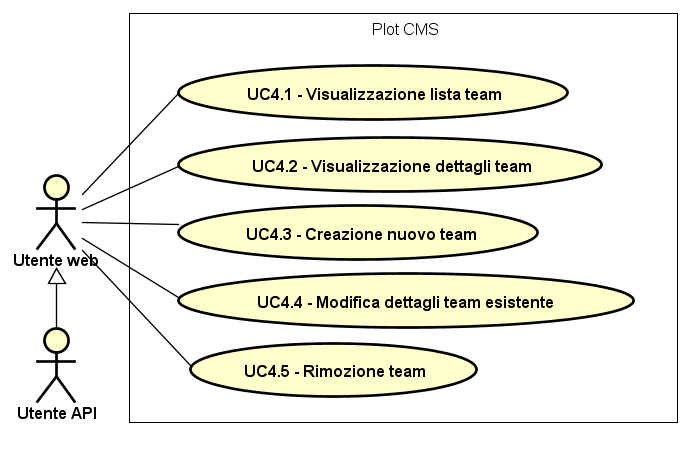
\includegraphics[scale=0.95, width=\textwidth]{immagini/usecase/UC4.png}
            \caption{Caso d'uso UC4: gestione team}\label{fig:UC4} 
        \end{figure}
\begin{itemize}
\item \textbf{Attori}: utente web, utente API;
\item \textbf{Descrizione}: un utente autenticato deve poter gestire gli aspetti di base legati ai team: creazione, visualizzazione, modifica e rimozione; 
      \item \textbf{Precondizione}: l'utente accede alla piattaforma attraverso un browser web o attraverso le API REST esposte dal sistema;

        \item \textbf{Flusso principale degli eventi}:
          \begin{enumerate}
          \item L'utente autenticato può visualizzare la lista dei team (\hyperlink{UC4.1}{UC4.1});
          \item L'utente autenticato può visualizzare i dettagli di uno specifico team (\hyperlink{UC4.2}{UC4.2});
          \item L'utente autenticato può creare un team (\hyperlink{UC4.3}{UC4.3});
          \item L'utente autenticato può modificare i dettagli di uno specifico team (\hyperlink{UC4.4}{UC4.4});
          \item L'utente autenticato può rimuovere un team (\hyperlink{UC4.5}{UC4.5}).

      \end{enumerate}
    \item \textbf{Postcondizione}: il sistema ha erogato le funzionalità richieste dall'utente.
  \end{itemize}
\hypertarget{UC4.1}{}
\section{Caso d'uso UC4.1: visualizzazione lista team}
\begin{itemize}
\item \textbf{Attori}: utente web, utente API;
\item \textbf{Descrizione}: l'utente autenticato deve poter visualizzare una lista di tutti i team in gioco. Ogni team deve riportare il numero di componenti e il punteggio totale, ovvero la somma dei punteggi ottenuti nelle mission disputate; 
      \item \textbf{Precondizione}: l'utente autenticato accede alla piattaforma attraverso un browser web o attraverso le API REST esposte dal sistema;

        \item \textbf{Flusso principale degli eventi}:
          \begin{enumerate}
          \item L'utente autenticato visualizza la lista dei team in gioco.

      \end{enumerate}
    \item \textbf{Postcondizione}: il sistema mostra la lista dei team in gioco.
  \end{itemize}
\hypertarget{UC4.2}{}
\section{Caso d'uso UC4.2: visualizzazione dettagli team}
\begin{itemize}
\item \textbf{Attori}: utente web, utente API;
\item \textbf{Descrizione}: l'utente autenticato deve poter visualizzare i dettagli relativi ad uno specifico team in gioco; 
      \item \textbf{Precondizione}: l'utente accede alla piattaforma attraverso un browser web o attraverso le API REST esposte dal sistema. Il team che si vuole visualizzare deve esistere;

        \item \textbf{Flusso principale degli eventi}:
          \begin{enumerate}
          \item L'utente autenticato visualizza il nome del team;
          \item L'utente autenticato visualizza l'URL dell'immagine rappresentativa del team;
          \item L'utente autenticato visualizza la lista degli utenti del gioco appartenenti al team.

      \end{enumerate}
    \item \textbf{Postcondizione}: il sistema mostra all'utente i dettagli del team richiesto.
  \end{itemize}
\hypertarget{UC4.3}{}
\section{Caso d'uso UC4.3: creazione nuovo team}
\begin{itemize}
\item \textbf{Attori}: utente web, utente API;
\item \textbf{Descrizione}: l'utente autenticato deve poter creare un nuovo team di gioco; 
      \item \textbf{Precondizione}: l'utente accede alla piattaforma attraverso un browser web o attraverso le API REST esposte dal sistema;

        \item \textbf{Flusso principale degli eventi}:
          \begin{enumerate}
          \item L'utente autenticato inserisce il nome del team;
          \item L'utente autenticato può inserire l'URL di un'immagine rappresentativa del team.

      \end{enumerate}
    \item \textbf{Postcondizione}: il sistema crea un nuovo team e ne mostra i dettagli all'utente.
  \end{itemize}
\hypertarget{UC4.4}{}
\section{Caso d'uso UC4.4: modifica dettagli team esistente}
\begin{itemize}
\item \textbf{Attori}: utente web, utente API;
\item \textbf{Descrizione}: l'utente autenticato deve poter modificare i dettagli relativi ad un team esistente; 
      \item \textbf{Precondizione}: l'utente accede alla piattaforma attraverso un browser web o attraverso le API REST esposte dal sistema. Il team che si vuole modificare deve esistere;

        \item \textbf{Flusso principale degli eventi}:
          \begin{enumerate}
          \item L'utente autenticato può modificare il nome del team;
          \item L'utente autenticato può modificare l'URL dell'immagine rappresentativa del team.

      \end{enumerate}
    \item \textbf{Postcondizione}: il sistema apporta le modifiche richieste e mostra i dettagli del team modificato all'utente.
  \end{itemize}
\hypertarget{UC4.5}{}
\section{Caso d'uso UC4.5: rimozione team}
\begin{itemize}
\item \textbf{Attori}: utente web, utente API;
\item \textbf{Descrizione}: l'utente autenticato deve poter rimuovere un team di gioco; 
      \item \textbf{Precondizione}: l'utente autenticato accede alla piattaforma attraverso un browser web o attraverso le API REST esposte dal sistema. Il team che si vuole rimuovere deve esistere;

        \item \textbf{Flusso principale degli eventi}:
          \begin{enumerate}
          \item L'utente autenticato rimuove un particolare team di gioco	.

      \end{enumerate}
    \item \textbf{Postcondizione}: Il team viene rimosso dal sistema e non può più essere recuperato. Il sistema mostra all'utente una lista degi team ancora presenti nel sistema.
  \end{itemize}
\hypertarget{UC5}{}
\section{Caso d'uso UC5: gestione admin}

        \begin{figure}
            \centering
            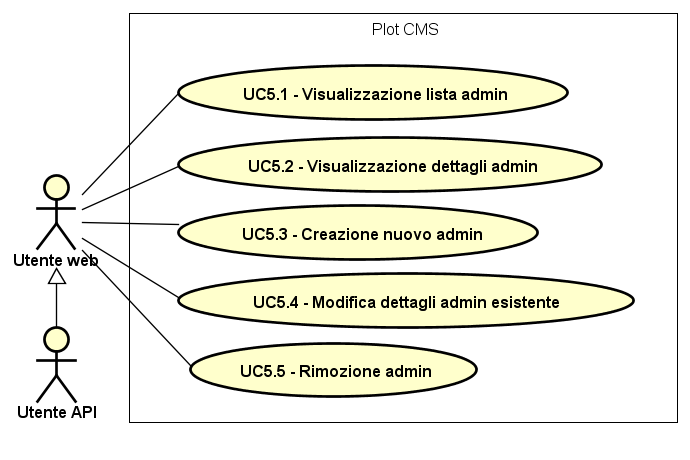
\includegraphics[scale=0.95, width=\textwidth]{immagini/usecase/UC5.png}
            \caption{Caso d'uso UC5: gestione admin}\label{fig:UC5} 
        \end{figure}
\begin{itemize}
\item \textbf{Attori}: utente web, utente API;
\item \textbf{Descrizione}: un utente autenticato deve poter gestire gli aspetti di base legati agli amministratori della piattaforma: creazione, visualizzazione, modifica e rimozione; 
      \item \textbf{Precondizione}: l'utente accede alla piattaforma attraverso un browser web o attraverso le API REST esposte dal sistema;

        \item \textbf{Flusso principale degli eventi}:
          \begin{enumerate}
          \item L'utente autenticato può visualizzare la lista degli amministratori della piattaforma (\hyperlink{UC5.1}{UC5.1});
          \item L'utente autenticato può visualizzare i dettagli di uno specifico amministratore della piattaforma (\hyperlink{UC5.2}{UC5.2});
          \item L'utente autenticato può creare un nuovo amministratore della piattaforma (\hyperlink{UC5.3}{UC5.3});
          \item L'utente autenticato può modificare i dettagli di uno specifico amministratore della piattaforma (\hyperlink{UC5.4}{UC5.4});
          \item L'utente autenticato può rimuovere un amministratore della piattaforma (\hyperlink{UC5.5}{UC5.5}).

      \end{enumerate}
    \item \textbf{Postcondizione}: il sistema ha erogato le funzionalità richieste dall'utente.
  \end{itemize}
\hypertarget{UC5.1}{}
\section{Caso d'uso UC5.1: visualizzazione lista admin}
\begin{itemize}
\item \textbf{Attori}: utente web, utente API;
\item \textbf{Descrizione}: l'utente autenticato deve poter visualizzare una lista di tutti gli amministratori della piattaforma. Gli amministratori sono coloro che possono utilizzare le funzionalità offerte dalla piattaforma; 
      \item \textbf{Precondizione}: l'utente autenticato accede alla piattaforma attraverso un browser web o attraverso le API REST esposte dal sistema;

        \item \textbf{Flusso principale degli eventi}:
          \begin{enumerate}
          \item L'utente autenticato visualizza la lista degli amministratori della piattaforma.

      \end{enumerate}
    \item \textbf{Postcondizione}: il sistema mostra la lista degli amministratori della piattaforma.
  \end{itemize}
\hypertarget{UC5.2}{}
\section{Caso d'uso UC5.2: visualizzazione dettagli admin}
\begin{itemize}
\item \textbf{Attori}: utente web, utente API;
\item \textbf{Descrizione}: l'utente autenticato deve poter visualizzare i dettagli relativi ad uno specifico amministratore della piattaforma; 
      \item \textbf{Precondizione}: l'utente accede alla piattaforma attraverso un browser web o attraverso le API REST esposte dal sistema. L'amministratore che si vuole visualizzare deve esistere;

        \item \textbf{Flusso principale degli eventi}:
          \begin{enumerate}
          \item L'utente autenticato visualizza il nome dell'amministratore della piattaforma;
          \item L'utente autenticato visualizza il cognome dell'amministratore della piattaforma;
          \item L'utente autenticato visualizza l'email dell'amministratore della piattaforma.

      \end{enumerate}
    \item \textbf{Postcondizione}: il sistema mostra all'utente i dettagli dell'amministratore richiesto.
  \end{itemize}
\hypertarget{UC5.3}{}
\section{Caso d'uso UC5.3: creazione nuovo admin}
\begin{itemize}
\item \textbf{Attori}: utente web, utente API;
\item \textbf{Descrizione}: l'utente autenticato deve poter creare un nuovo amministratore della piattaforma ; 
      \item \textbf{Precondizione}: l'utente accede alla piattaforma attraverso un browser web o attraverso le API REST esposte dal sistema;

        \item \textbf{Flusso principale degli eventi}:
          \begin{enumerate}
          \item L'utente autenticato inserisce il nome dell'amministratore della piattaforma;
          \item L'utente autenticato inserisce il cognome dell'amministratore della piattaforma;
          \item L'utente autenticato inserisce l'email dell'amministratore della piattaforma;
          \item L'utente autenticato inserisce la password dell'amministratore della piattaforma.

      \end{enumerate}
    \item \textbf{Postcondizione}: il sistema crea un nuovo amministratore della piattaforma e ne mostra i dettagli all'utente.
  \end{itemize}
\hypertarget{UC5.4}{}
\section{Caso d'uso UC5.4: modifica dettagli admin esistente}
\begin{itemize}
\item \textbf{Attori}: utente web, utente API;
\item \textbf{Descrizione}: l'utente autenticato deve poter modificare i dettagli relativi ad un amministratore esistente; 
      \item \textbf{Precondizione}: l'utente accede alla piattaforma attraverso un browser web o attraverso le API REST esposte dal sistema. L'amministratore che si vuole modificare deve esistere;

        \item \textbf{Flusso principale degli eventi}:
          \begin{enumerate}
          \item L'utente autenticato può modificare il nome dell'amministratore;
          \item L'utente autenticato può modificare il cognome dell'amministratore;
          \item L'utente autenticato può modificare l'email dell'amministratore.

      \end{enumerate}
    \item \textbf{Postcondizione}: il sistema apporta le modifiche richieste e mostra i dettagli dell'amministratore modificato all'utente.
  \end{itemize}
\hypertarget{UC5.5}{}
\section{Caso d'uso UC5.5: rimozione admin}
\begin{itemize}
\item \textbf{Attori}: utente web, utente API;
\item \textbf{Descrizione}: l'utente autenticato deve poter rimuovere un amministratore della piattaforma; 
      \item \textbf{Precondizione}: l'utente autenticato accede alla piattaforma attraverso un browser web o attraverso le API REST esposte dal sistema. L'amministratore che si vuole rimuovere deve esistere;

        \item \textbf{Flusso principale degli eventi}:
          \begin{enumerate}
          \item L'utente autenticato rimuove un particolare amministratore della piattaforma.

      \end{enumerate}
    \item \textbf{Postcondizione}: l'amministratore viene rimosso dal sistema e non può più essere recuperato. Il sistema mostra all'utente una lista degli amministratori ancora presenti nel sistema.
  \end{itemize}
\hypertarget{UC6}{}
\section{Caso d'uso UC6: gestione log}

        \begin{figure}[H]
            \centering
            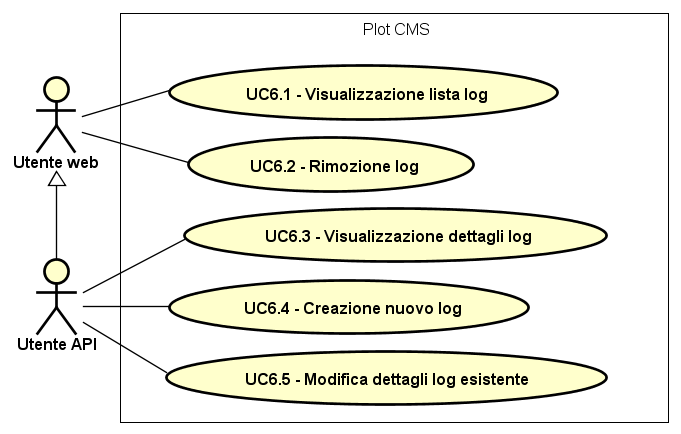
\includegraphics[scale=0.95, width=\textwidth]{immagini/usecase/UC6.png}
            \caption{Caso d'uso UC6: gestione log}\label{fig:UC6} 
        \end{figure}
\begin{itemize}
\item \textbf{Attori}: utente web, utente API;
\item \textbf{Descrizione}: un utente autenticato che accede alla piattaforma dal web deve poter gestire la visualizzazione e la rimozione dei log generati dagli utenti del gioco.
In aggiunta a ciò, un utente autenticato che accede alla piattaforma attraverso le API deve poter creare un nuovo log e modificare un log esistente; 
      \item \textbf{Precondizione}: l'utente accede alla piattaforma attraverso un browser web o attraverso le API REST esposte dal sistema;

        \item \textbf{Flusso principale degli eventi}:
          \begin{enumerate}
          \item L'utente autenticato che accede tramite web può visualizzare la lista dei log (\hyperlink{UC6.1}{UC6.1});
          \item L'utente autenticato che accede tramite web può rimuovere un log (\hyperlink{UC6.2}{UC6.2});
          \item L'utente autenticato che accede tramite API può visualizzare i dettagli di uno specifico log (\hyperlink{UC6.3}{UC6.3});
          \item L'utente autenticato che accede tramite API può creare un nuovo log (\hyperlink{UC6.4}{UC6.4});
          \item L'utente autenticato che accede tramite API può modificare i dettagli di uno specifico log (\hyperlink{UC6.5}{UC6.5}).

      \end{enumerate}
    \item \textbf{Postcondizione}: il sistema ha erogato le funzionalità richieste dall'utente.
  \end{itemize}
\hypertarget{UC6.1}{}
\section{Caso d'uso UC6.1: visualizzazione lista log}
\begin{itemize}
\item \textbf{Attori}: utente web, utente API;
\item \textbf{Descrizione}: l'utente autenticato deve poter visualizzare una lista di tutti i log generati dalle richieste HTTP effettuate dagli utenti di gioco ; 
      \item \textbf{Precondizione}: l'utente autenticato accede alla piattaforma attraverso un browser web o attraverso le API REST esposte dal sistema;

        \item \textbf{Flusso principale degli eventi}:
          \begin{enumerate}
          \item L'utente autenticato visualizza la lista dei log generati dalle richieste HTTP effettuate dagli utenti di gioco .

      \end{enumerate}
    \item \textbf{Postcondizione}: il sistema mostra la lista dei log generati dalle richieste HTTP effettuate dagli utenti di gioco .
  \end{itemize}
\hypertarget{UC6.2}{}
\section{Caso d'uso UC6.2: rimozione log}
\begin{itemize}
\item \textbf{Attori}: utente web, utente API;
\item \textbf{Descrizione}: l'utente autenticato deve poter rimuovere un log generato da una richiesta HTTP effettuata da un utente di gioco; 
      \item \textbf{Precondizione}: l'utente autenticato accede alla piattaforma attraverso un browser web o attraverso le API REST esposte dal sistema. Il log che si vuole rimuovere deve esistere;

        \item \textbf{Flusso principale degli eventi}:
          \begin{enumerate}
          \item L'utente autenticato rimuove un log generato da una richiesta HTTP effettuata da un utente di gioco.

      \end{enumerate}
    \item \textbf{Postcondizione}: il log viene rimosso dal sistema e non può più essere recuperato. Il sistema mostra all'utente una lista dei log ancora presenti nel sistema.
  \end{itemize}
\hypertarget{UC6.3}{}
\section{Caso d'uso UC6.3: visualizzazione dettagli log}
\begin{itemize}
\item \textbf{Attori}: utente API;
\item \textbf{Descrizione}: l'utente autenticato deve poter visualizzare i dettagli di un log generato da una richiesta HTTP effettuata da un utente di gioco; 
      \item \textbf{Precondizione}: l'utente autenticato accede alla piattaforma attraverso le API REST esposte dal sistema. Il log che si vuole visualizzare deve esistere;

        \item \textbf{Flusso principale degli eventi}:
          \begin{enumerate}
          \item L'utente autenticato visualizza l'utente di gioco che ha effettuato la richiesta HTTP;
          \item L'utente autenticato visualizza il metodo HTTP utilizzato per la richiesta;
          \item L'utente autenticato visualizza l'URL alla quale è stata inoltrata la richiesta HTTP;
          \item L'utente autenticato visualizza lo user agent utilizzato per inoltrare la richiesta HTTP;
          \item L'utente autenticato visualizza l'indirizzo IP che ha effettuato la richiesta HTTP;
          \item L'utente autenticato visualizza i dati aggiuntivi trasportati dalla richiesta HTTP;
          \item L'utente autenticato visualizza il timestamp relativo alla creazione del log.

      \end{enumerate}
    \item \textbf{Postcondizione}: i dettagli del log vengono mostrati all'utente.
  \end{itemize}
\hypertarget{UC6.4}{}
\section{Caso d'uso UC6.4: creazione nuovo log}
\begin{itemize}
\item \textbf{Attori}: utente API;
\item \textbf{Descrizione}: l'utente autenticato deve poter creare un nuovo log utilizzando i dettagli di da una richiesta HTTP effettuata da un utente di gioco; 
      \item \textbf{Precondizione}: l'utente autenticato accede alla piattaforma attraverso le API REST esposte dal sistema. Il log che si vuole visualizzare deve esistere;

        \item \textbf{Flusso principale degli eventi}:
          \begin{enumerate}
          \item L'utente autenticato inserisce l'user che ha effettuato la richiesta HTTP;
          \item L'utente autenticato inserisce il metodo HTTP utilizzato per la richiesta;
          \item L'utente autenticato inserisce l'URL indirizzato dalla richiesta HTTP;
          \item L'utente autenticato inserisce lo user agent che ha effettuato la richiesta HTTP;
          \item L'utente autenticato inserisce l'indirizzo IP che ha effettuato la richiesta HTTP;
          \item L'utente autenticato inserisce i dati aggiuntivi trasportati dalla la richiesta HTTP;
          \item L'utente autenticato inserisce il timestamp relativo alla creazione del corrente log.

      \end{enumerate}
    \item \textbf{Postcondizione}: Il sistema crea un nuovo log e ne mostra i dettagli all'utente.
  \end{itemize}
\hypertarget{UC6.5}{}
\section{Caso d'uso UC6.5: modifica dettagli log esistente}
\begin{itemize}
\item \textbf{Attori}: utente API;
\item \textbf{Descrizione}: l'utente autenticato deve poter modificare log esistente ; 
      \item \textbf{Precondizione}: l'utente autenticato accede alla piattaforma attraverso le API REST esposte dal sistema. Il log che si vuole modificare deve esistere;

        \item \textbf{Flusso principale degli eventi}:
          \begin{enumerate}
          \item L'utente autenticato può modificare l'user che ha effettuato la richiesta HTTP;
          \item L'utente autenticato può modificare il metodo HTTP utilizzato per la richiesta;
          \item L'utente autenticato può modificare l'URL indirizzato dalla richiesta HTTP;
          \item L'utente autenticato può modificare lo user agent che ha effettuato la richiesta HTTP;
          \item L'utente autenticato può modificare l'indirizzo IP che ha effettuato la richiesta HTTP;
          \item L'utente autenticato può modificare i dati aggiuntivi trasportati dalla la richiesta HTTP;
          \item L'utente autenticato può modificare il timestamp relativo alla creazione del corrente log;
          \item L'utente autenticato può modificare il timestamp relativo alla creazione del corrente log;
          \item L'utente autenticato può modificare il timestamp relativo alla creazione del corrente log.

      \end{enumerate}
    \item \textbf{Postcondizione}: Il sistema apporta le modifiche richieste e mostra i dettagli del log modificato all'utente.
  \end{itemize}



             % Appendice A

%**************************************************************
% Materiale finale
%**************************************************************
\backmatter
\printglossaries
% !TEX encoding = UTF-8
% !TEX TS-program = pdflatex
% !TEX root = ../tesi.tex
% !TEX spellcheck = it-IT

%**************************************************************
% Bibliografia
%**************************************************************

\cleardoublepage
\chapter{Bibliografia}

\nocite{*}
%\printbibliography

\bibbycategory % equivale a dare un \printbibliography per ogni categoria


\end{document}